% !TEX root = ../optim-ml/OptimML.tex

%%%%%%%%%%%%%%%%%%%%%%%%%%%%%%%%%%%%%%%%%%%%%%%%%%%%%%%%%%%%%%%%%%%%%%%%%%%%%%%%%%
%%%%%%%%%%%%%%%%%%%%%%%%%%%%%%%%%%%%%%%%%%%%%%%%%%%%%%%%%%%%%%%%%%%%%%%%%%%%%%%%%%
%%%%%%%%%%%%%%%%%%%%%%%%%%%%%%%%%%%%%%%%%%%%%%%%%%%%%%%%%%%%%%%%%%%%%%%%%%%%%%%%%%
\section{Motivation in Machine Learning}

%%%%%%%%%%%%%%%%%%%%%%%%%%%%%%%%%%%%%%%%%%%%%%%%%%%%%%%%%%%%%%%%%%%%%%%%%%%%%%%%%%
\subsection{Unconstraint optimization}

In most part of this Chapter, we consider unconstrained convex optimization problems of the form 
\eql{\label{eq-general-pbm} 
	\uinf{x \in \RR^p} f(x),
}
and try to devise ``cheap'' algorithms with a low computational cost per iteration to approximate a minimizer when it exists. 
%
The class of algorithms considered are first order, i.e. they make use of gradient information. In the following, we denote 
\eq{
	\uargmin{x} f(x) \eqdef \enscond{x \in \RR^p}{ f(x) = \inf{f}}, 
} 
to indicate the set of points (it is not necessarily a singleton since the minimizer might be non-unique) that achieve the minimum of the function $f$. One might have $\argmin f = \emptyset$ (this situation is discussed below), but in case a minimizer exists, we denote the optimization problem as
\eql{\label{eq-general-pbm-min} 
	\umin{x \in \RR^p} f(x).
}


In typical learning scenario, $f(x)$ is the empirical risk for regression or classification, and $p$ is the number of parameter. For instance, in the simplest case of linear models, we denote $(a_i,y_i)_{i=1}^n$ where $a_i \in \RR^p$ are the features. 
%
In the following, we denote $A \in \RR^{n \times p}$ the matrix whose rows are the $a_i$.


\begin{figure}
\centering
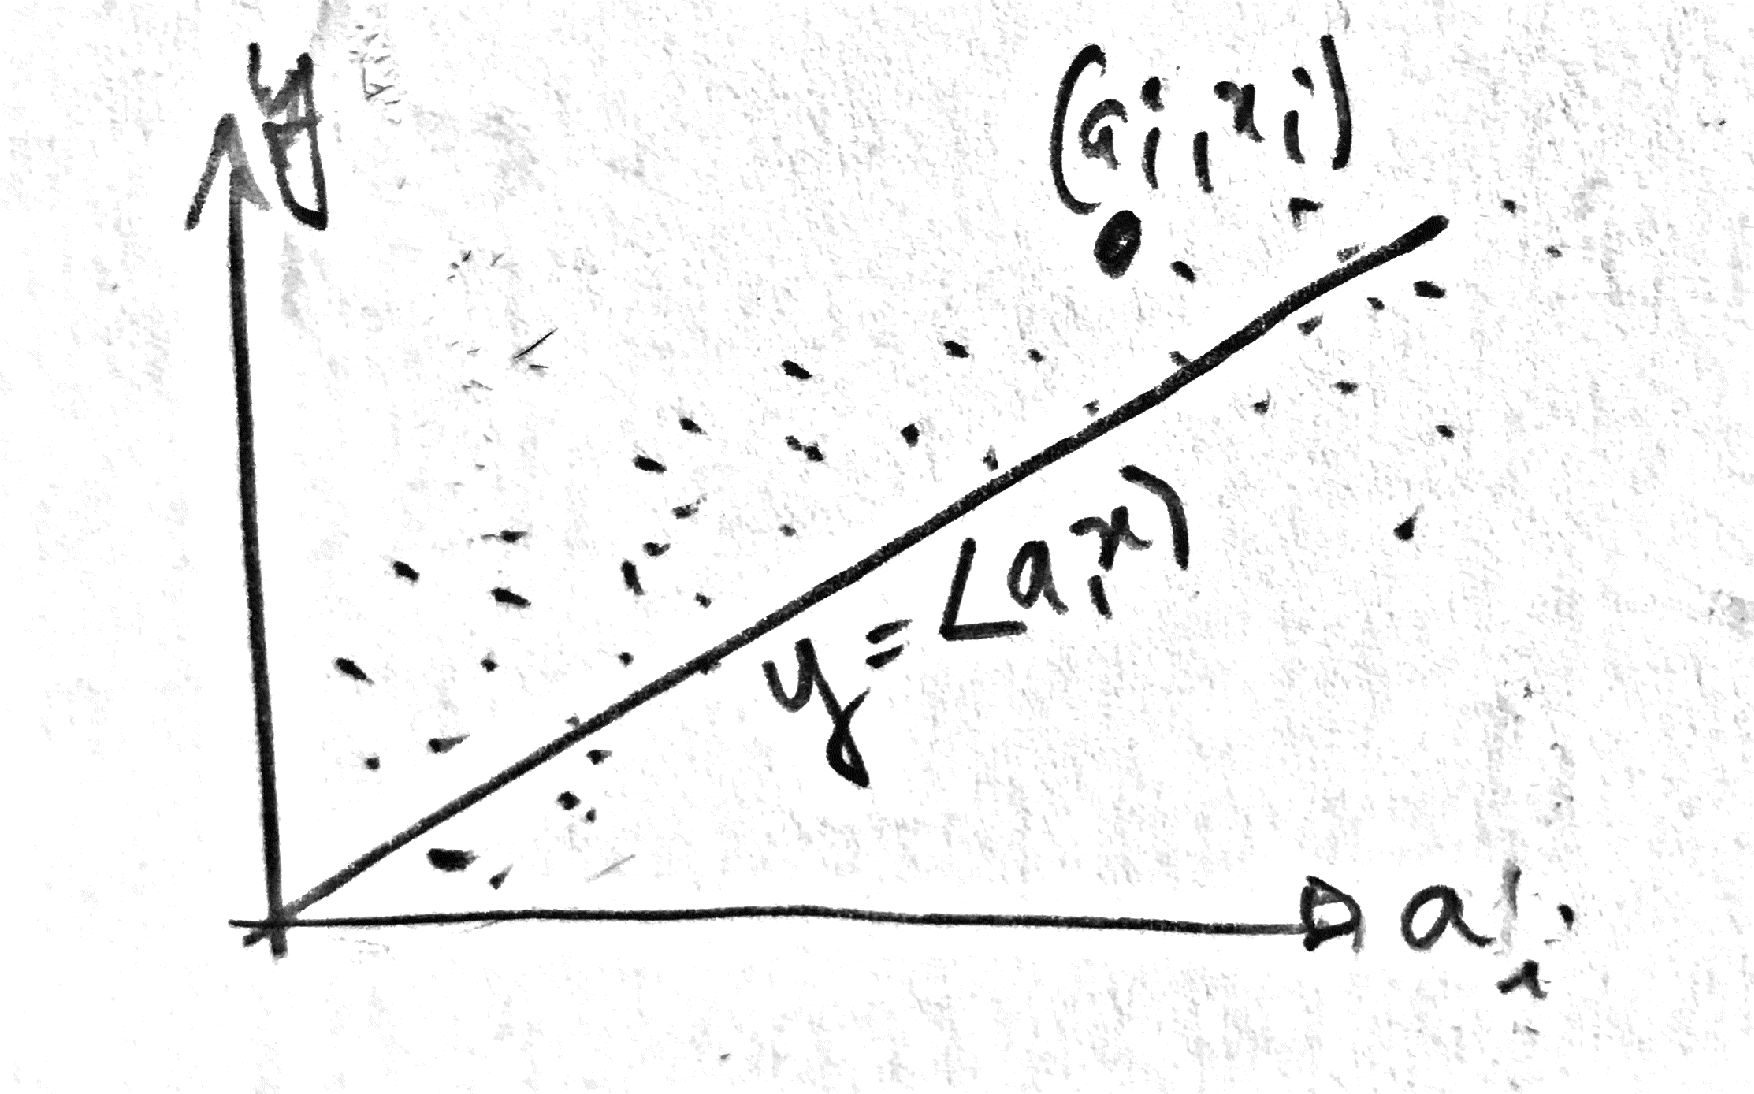
\includegraphics[width=.2\linewidth]{optim-smooth/ml-exemp-1} \quad
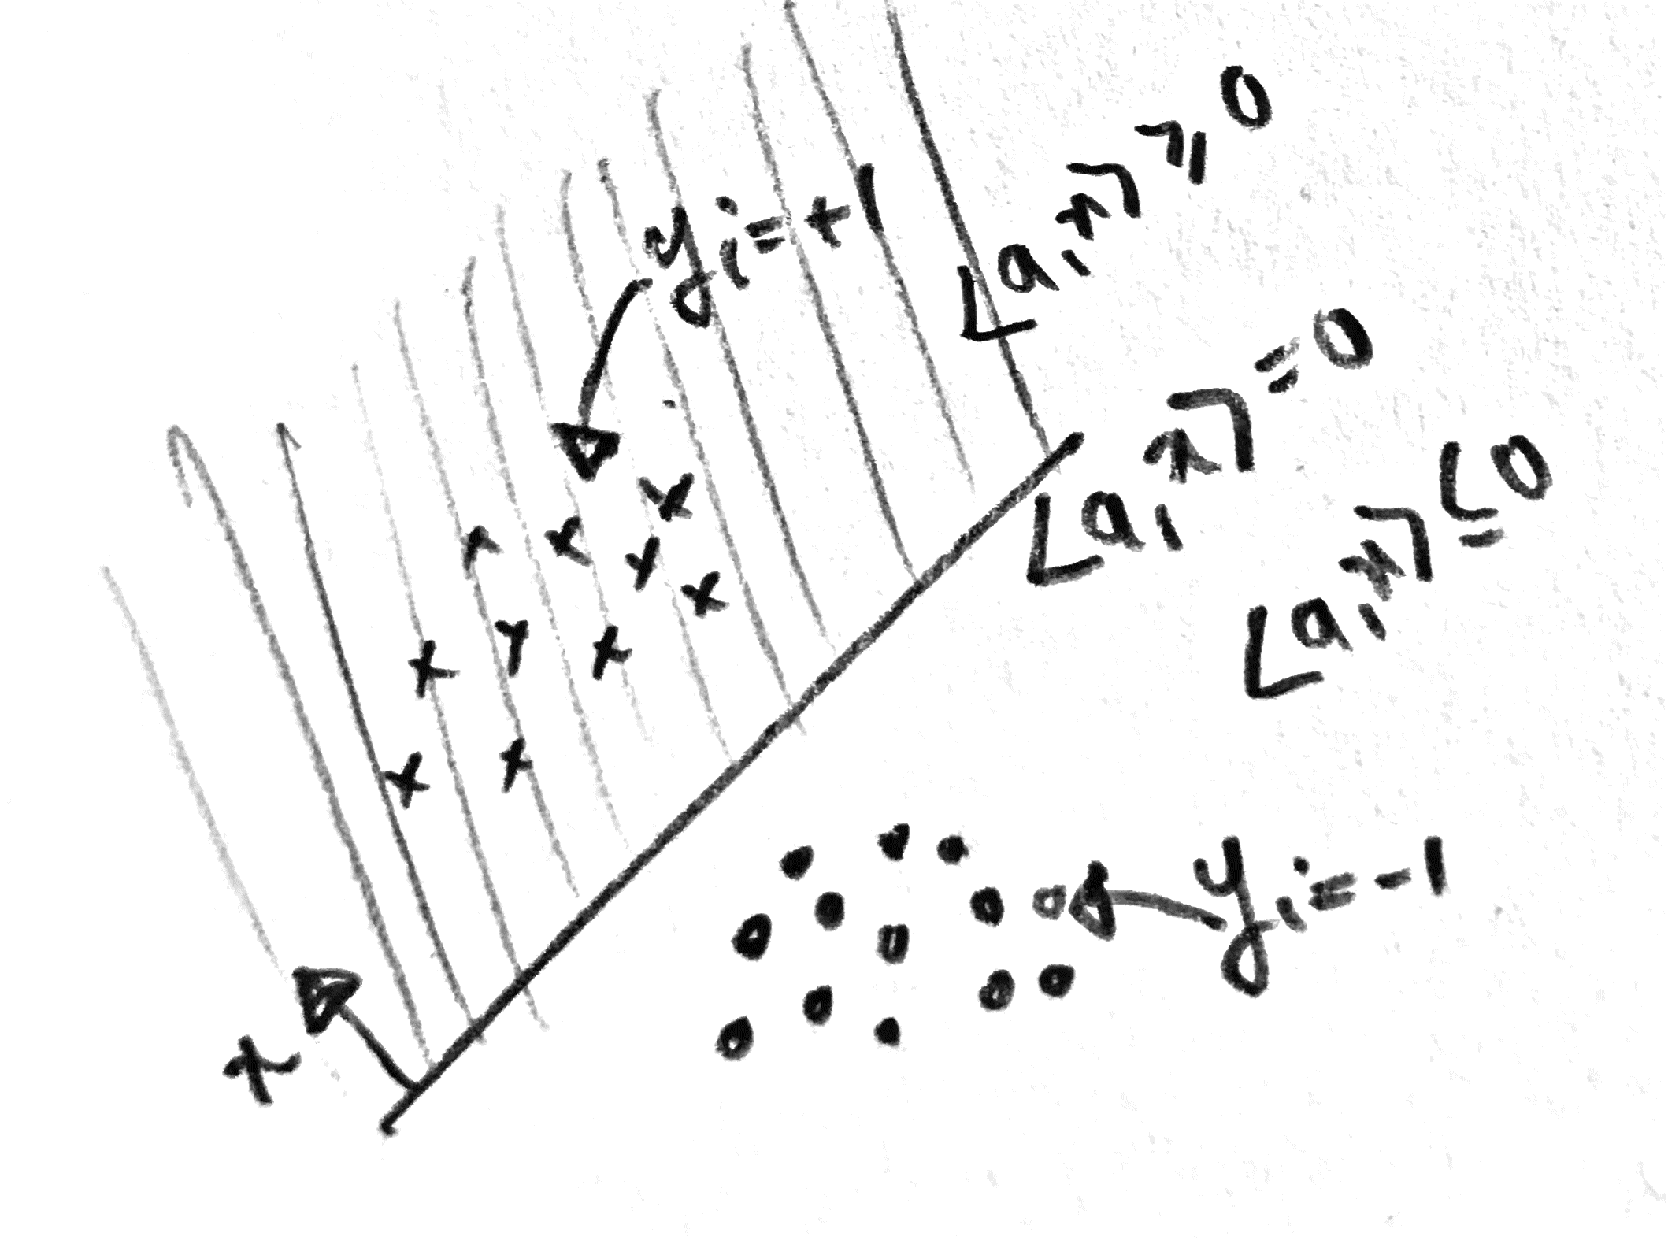
\includegraphics[width=.2\linewidth]{optim-smooth/ml-exemp-2} \quad
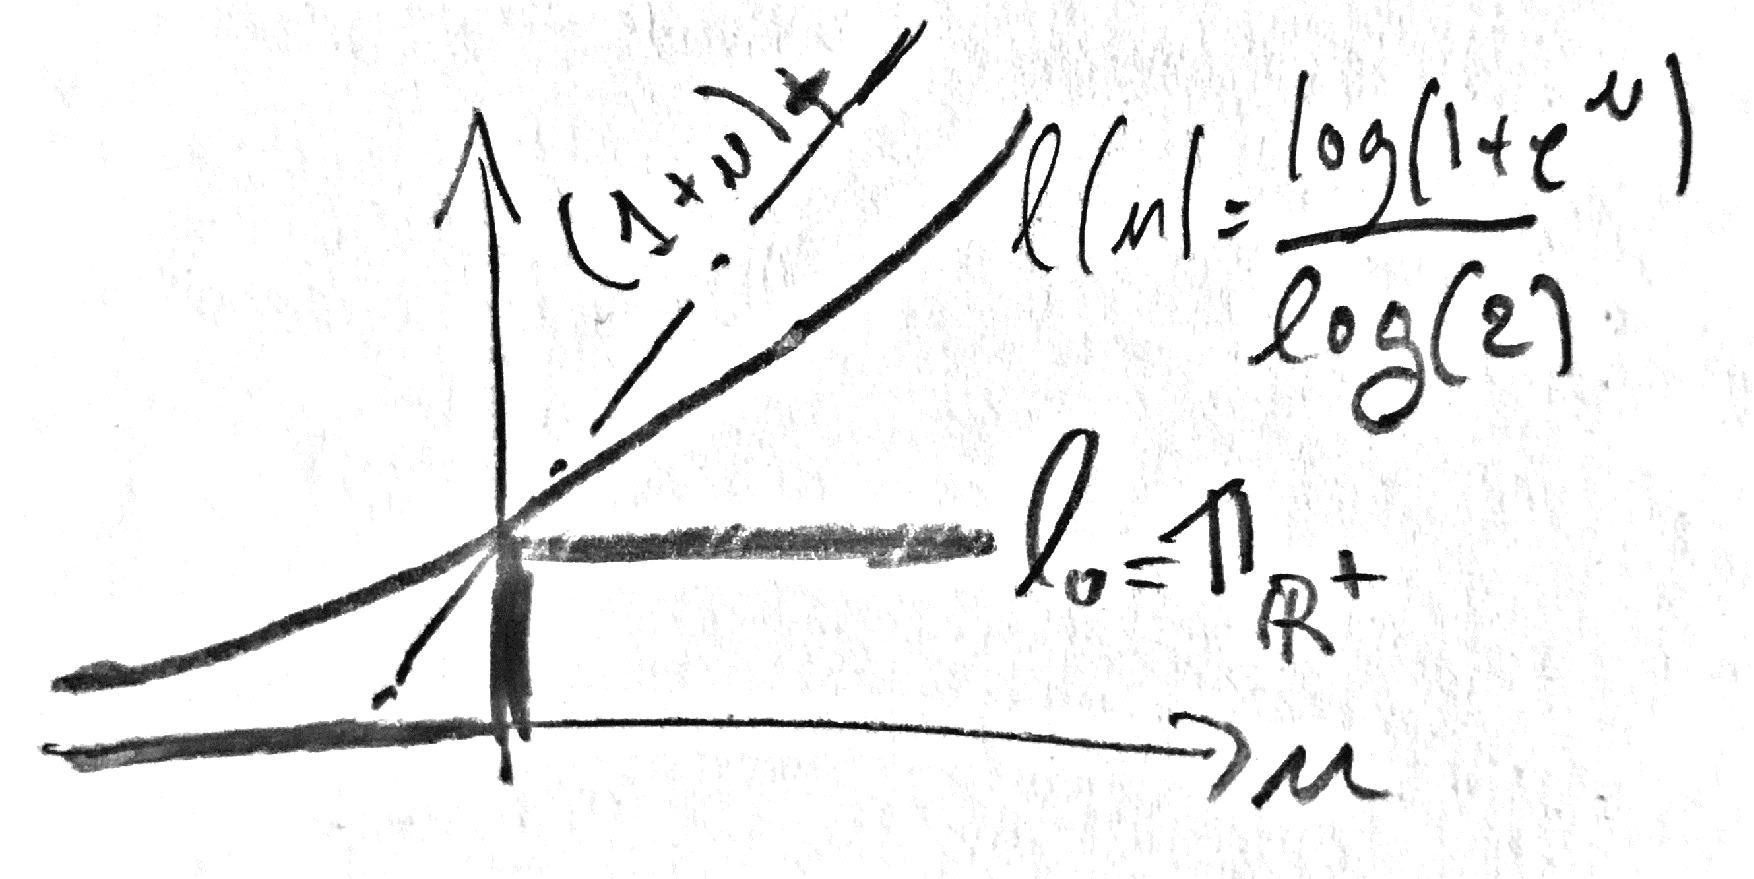
\includegraphics[width=.3\linewidth]{optim-smooth/classif-loss}
\caption{\label{fig-ml-ex}
Left: linear regression, middle: linear classifier, right: loss function for classification.
}
\end{figure}


%%%%%%%%%%%%%%%%%%%%%%%%%%%%%%%%%%%%%%%%%%%%%%%%%%%%%%%%%%%%%%%%%%%%%%%%%%%%%%%%%%
\subsection{Regression}

For regression, $y_i \in \RR$, in which case
\eql{\label{eq-least-square}
	f(x) =  \frac{1}{2}\sum_{i=1}^n (y_i-\dotp{x}{a_i})^2 = \frac{1}{2}\norm{Ax-y}^2, 
} 
is the least square quadratic risk function (see Fig.~\ref{fig-ml-ex}).
%
Here $\dotp{u}{v}=\sum_{i=1}^p u_i v_i$ is the canonical inner product in $\RR^p$ and $\norm{\cdot}^2=\dotp{\cdot}{\cdot}$. 


%%%%%%%%%%%%%%%%%%%%%%%%%%%%%%%%%%%%%%%%%%%%%%%%%%%%%%%%%%%%%%%%%%%%%%%%%%%%%%%%%%
\subsection{Classification}

For classification, $y_i \in \{-1,1\}$, in which case
\eql{\label{eq-classif}
	f(x) = \sum_{i=1}^n \ell(-y_i \dotp{x}{a_i}) = L( - \diag(y) A x )
}
where $\ell$ is a smooth approximation of the 0-1 loss $1_{\RR^+}$.
%
For instance $\ell(u)=\log(1+\exp(u))$, and $\diag(y) \in \RR^{n \times n}$ is the diagonal matrix with $y_i$ along the diagonal (see Fig.~\ref{fig-ml-ex}, right). Here the separable loss function $L = \RR^n \rightarrow \RR$ is, for $z \in \RR^n$, $L(z)=\sum_i \ell(z_i)$. 


%%%%%%%%%%%%%%%%%%%%%%%%%%%%%%%%%%%%%%%%%%%%%%%%%%%%%%%%%%%%%%%%%%%%%%%%%%%%%%%%%%
%%%%%%%%%%%%%%%%%%%%%%%%%%%%%%%%%%%%%%%%%%%%%%%%%%%%%%%%%%%%%%%%%%%%%%%%%%%%%%%%%%
%%%%%%%%%%%%%%%%%%%%%%%%%%%%%%%%%%%%%%%%%%%%%%%%%%%%%%%%%%%%%%%%%%%%%%%%%%%%%%%%%%
\section{Basics of Convex Analysis}

%%%%%%%%%%%%%%%%%%%%%%%%%%%%%%%%%%%%%%%%%%%%%%%%%%%%%%%%%%%%%%%%%%%%%%%%%%%%%%%%%%
\subsection{Existence of Solutions}

In general, there might be no solution to the optimization~\eqref{eq-general-pbm}. This is of course the case if $f$ is unbounded by bellow, for instance $f(x)=-x^2$ in which case the value of the minimum is $-\infty$. But this might also happen if $f$ does not grow at infinity, for instance $f(x)=e^{-x}$, for which $\min f = 0$ but there is no minimizer.

\begin{figure}
\centering
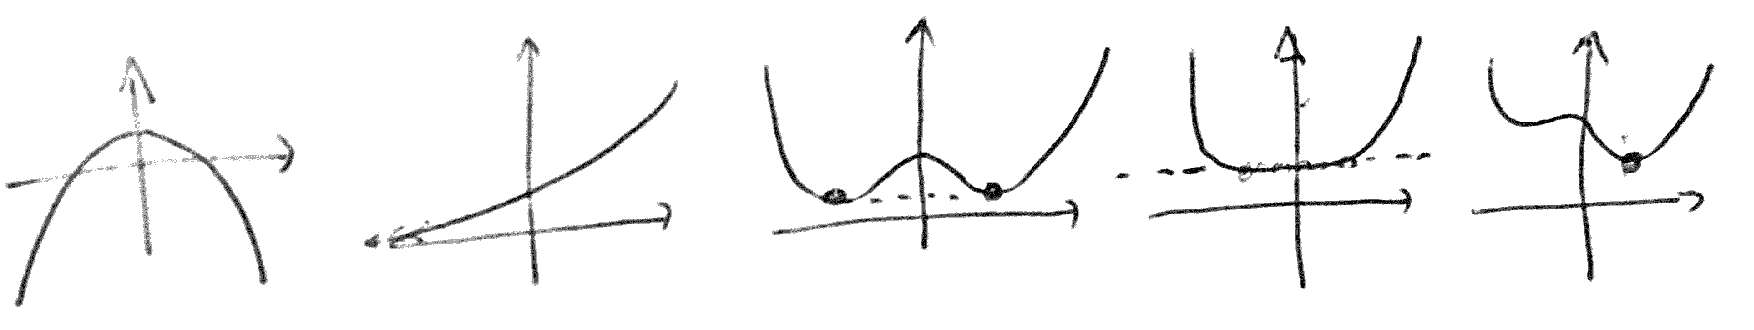
\includegraphics[width=.9\linewidth]{optim-smooth/uniqueness}
\caption{\label{fig-minimizer-exists}
Left: non-existence of minimizer, middle: multiple minimizers, right: uniqueness.
}
\end{figure}

In order to show existence of a minimizer, and that the set of minimizer is bounded (otherwise one can have problems with optimization algorithm that could escape to infinity), one needs to show that one can replace the whole space $\RR^p$ by a compact sub-set $\Om \subset \RR^p$ (i.e. $\Om$ is bounded and close) and that $f$ is continuous on $\Om$ (one can replace this by a weaker condition, that $f$ is lower-semi-continuous, but we ignore this here).  A way to show that one can consider only a bounded set is to show that $f(x) \rightarrow +\infty$ when $x \rightarrow +\infty$. Such a function is called coercive. In this case, one can choose any $x_0 \in \RR^p$ and consider its associated lower-level set
\eq{
	\Om = \enscond{x \in \RR^p}{f(x) \leq f(x_0)}
}
which is bounded because of coercivity, and closed because $f$ is continuous. One can actually show that for convex function, having a bounded set of minimizer is equivalent to the function being coercive (this is not the case for non-convex function, for instance $f(x)=\min(1,x^2)$ has a single minimum but is not coercive). 

\begin{figure}
\centering
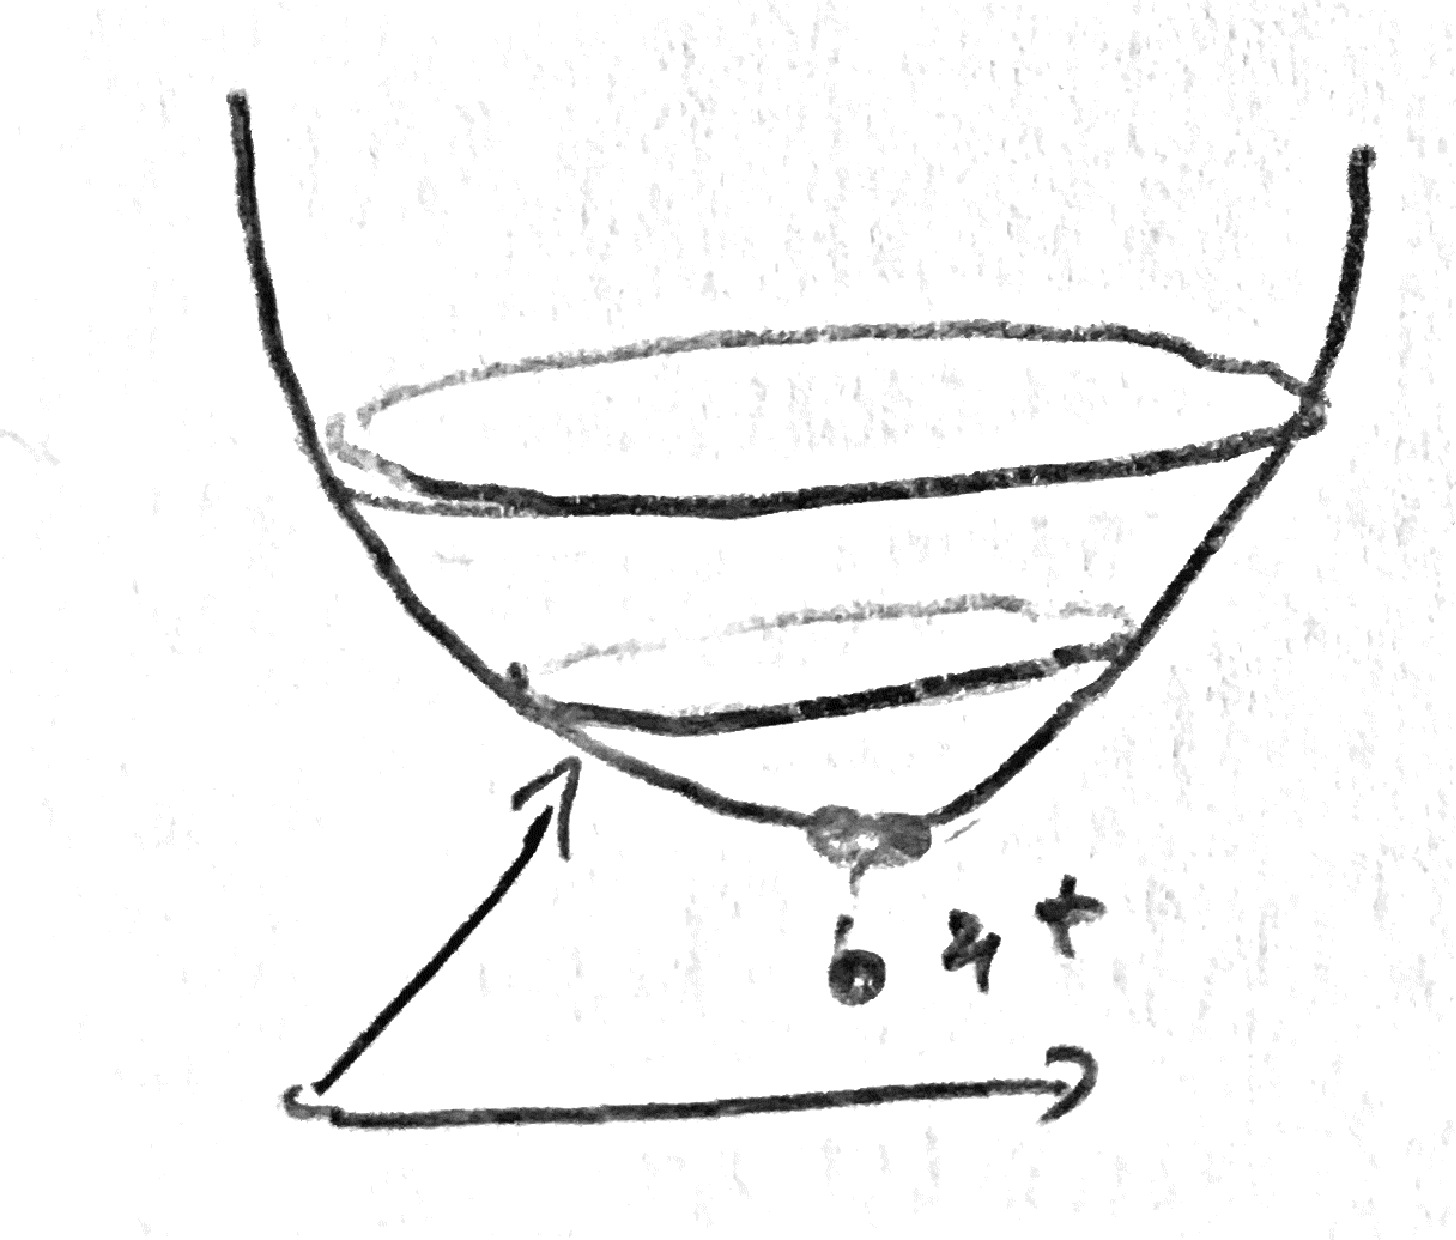
\includegraphics[width=.2\linewidth]{optim-smooth/least-square-1} \quad
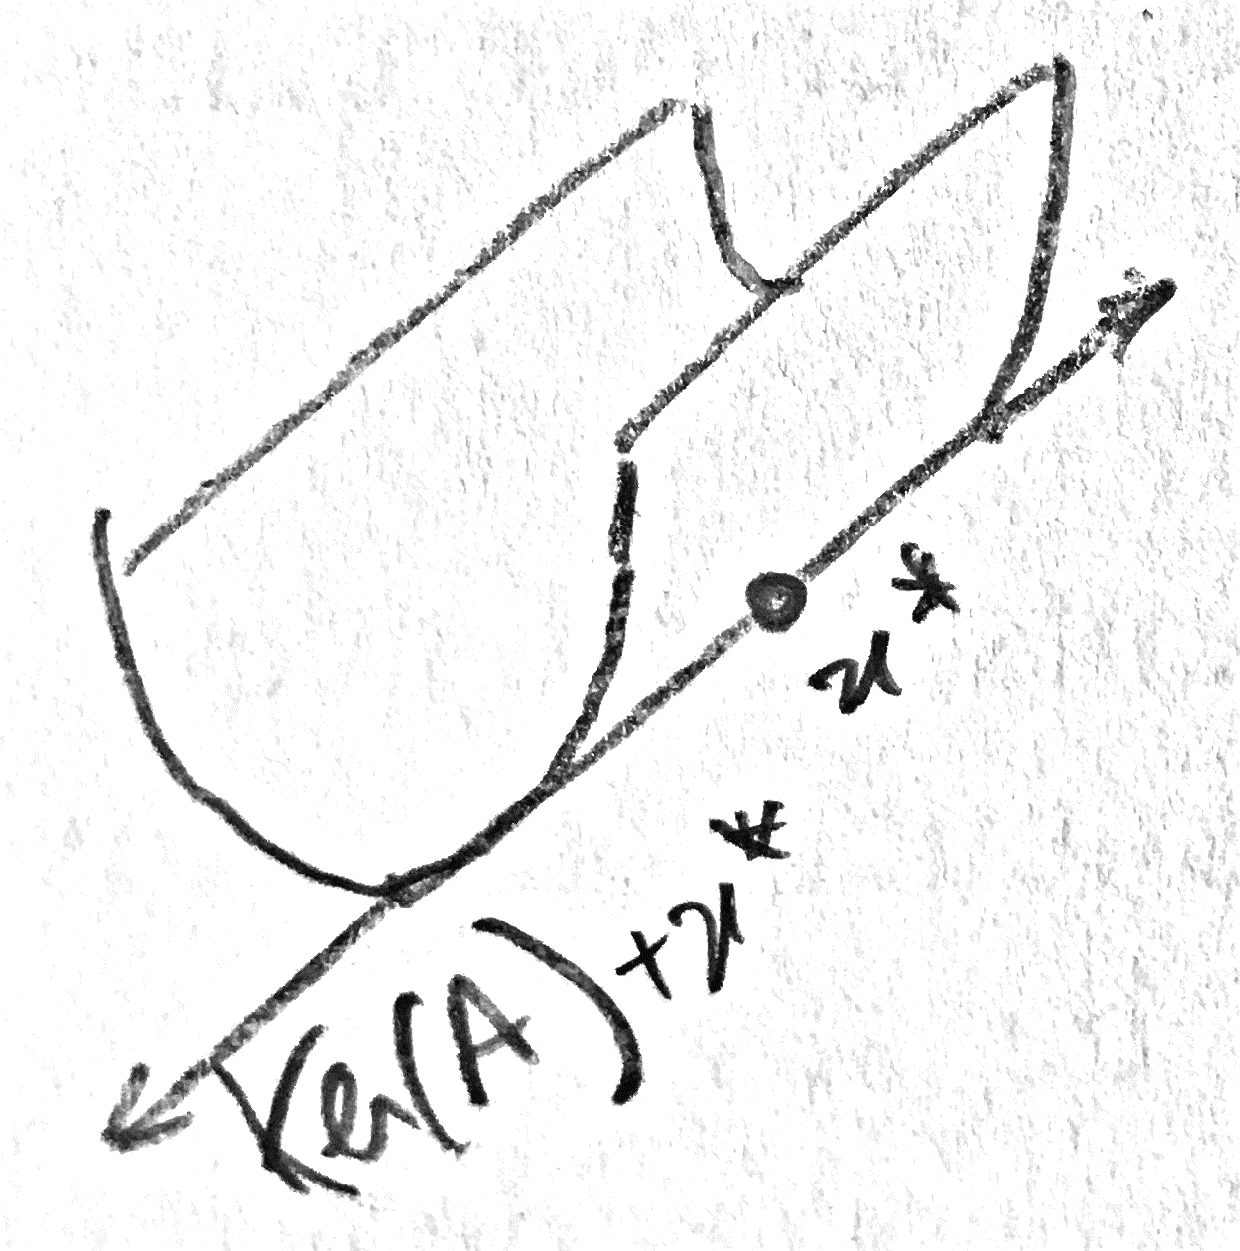
\includegraphics[width=.2\linewidth]{optim-smooth/least-square-2} 
\caption{\label{fig-least-square}
Coercivity condition for least squares.
}
\end{figure}

\begin{exmp}[Least squares]
For instance, for the quadratic loss function $f(x)=\frac{1}{2}\norm{Ax-y}^2$, coercivity holds if and only if $\ker(A)=\{0\}$ (this corresponds to the overdetermined setting). Indeed, if $\ker(A) \neq \{0\}$ if $x^\star$ is a solution, then $x^\star+u$ is also solution for any $u \in \ker(A)$, so that the set of minimizer is unbounded.
%
On contrary, if $\ker(A) = \{0\}$, we will show later that the set of minimizer is unique, see Fig.~\ref{fig-least-square}. 
%
If $\ell$ is strictly convex, the same conclusion holds in the case of classification.
\end{exmp}

%%%%%%%%%%%%%%%%%%%%%%%%%%%%%%%%%%%%%%%%%%%%%%%%%%%%%%%%%%%%%%%%%%%%%%%%%%%%%%%%%%
\subsection{Convexity}

Convex functions define the main class of functions which are somehow ``simple'' to optimize, in the sense that all minimizers are global minimizers, and that there are often efficient methods to find these minimizers (at least for smooth convex functions). A convex function is such that for any pair of point $(x,y) \in (\RR^p)^2$, 
\eql{\label{eq-convexity-def}
	\foralls t \in [0,1], \quad
		f((1-t)x + t y) \leq (1-t)f(x) + t f(y)
}
which means that the function is bellow its secant (and actually also above its tangent when this is well defined), see Fig.~\ref{fig-cvx-vs-noncvx}. 
%
If $x^\star$ is a local minimizer of a convex $f$, then $x^\star$ is a global minimizer, i.e. $x^\star \in \argmin f$.  


Convex function are very convenient because they are stable under lots of transformation. In particular, if $f$, $g$ are convex and $a, b$ are positive, $a f + b g$ is convex (the set of convex function is itself an infinite dimensional convex cone!) and so is $\max(f,g)$. If $g : \RR^q \rightarrow \RR$ is convex and $B \in \RR^{q \times p}, b \in \RR^q$ then $f(x) = g(B x+b)$ is convex. 
%
This shows immediately that the square loss appearing in~\eqref{eq-least-square} is convex, since $\norm{\cdot}^2/2$ is convex (as a sum of squares). 
%
Also, similarly, if $\ell$ and hence $L$ is convex, then the classification loss function~\eqref{eq-classif} is itself convex. 

\begin{figure}
\centering
\begin{tabular}{cccc}
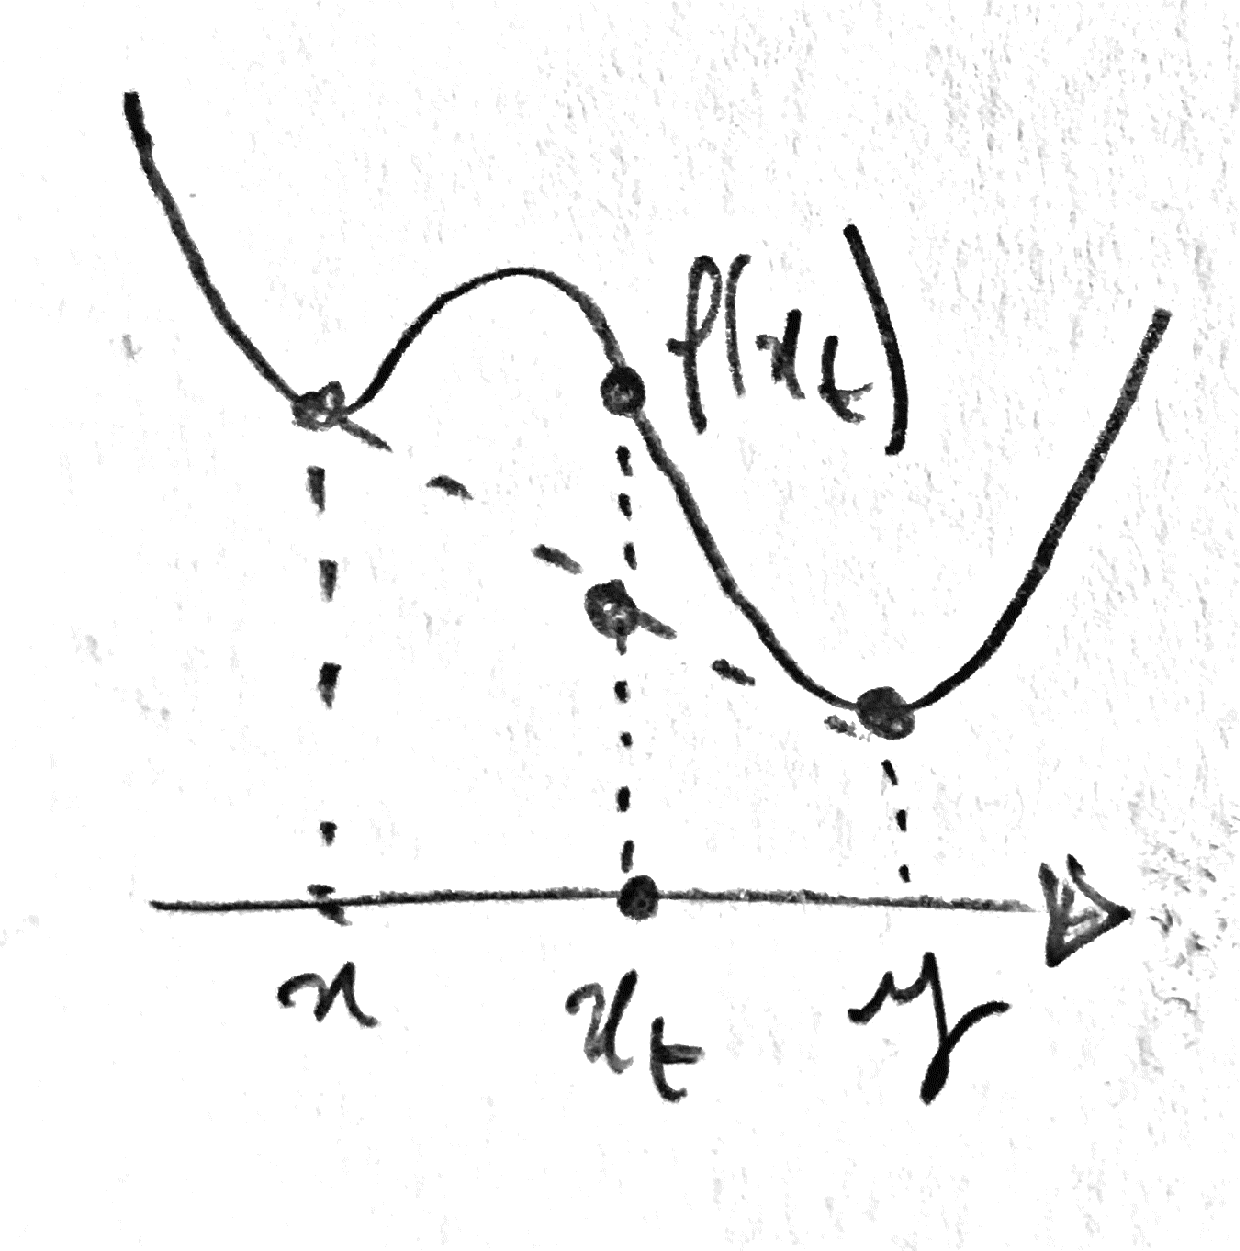
\includegraphics[width=.2\linewidth]{optim-smooth/cvx-vs-noncvx-1} &
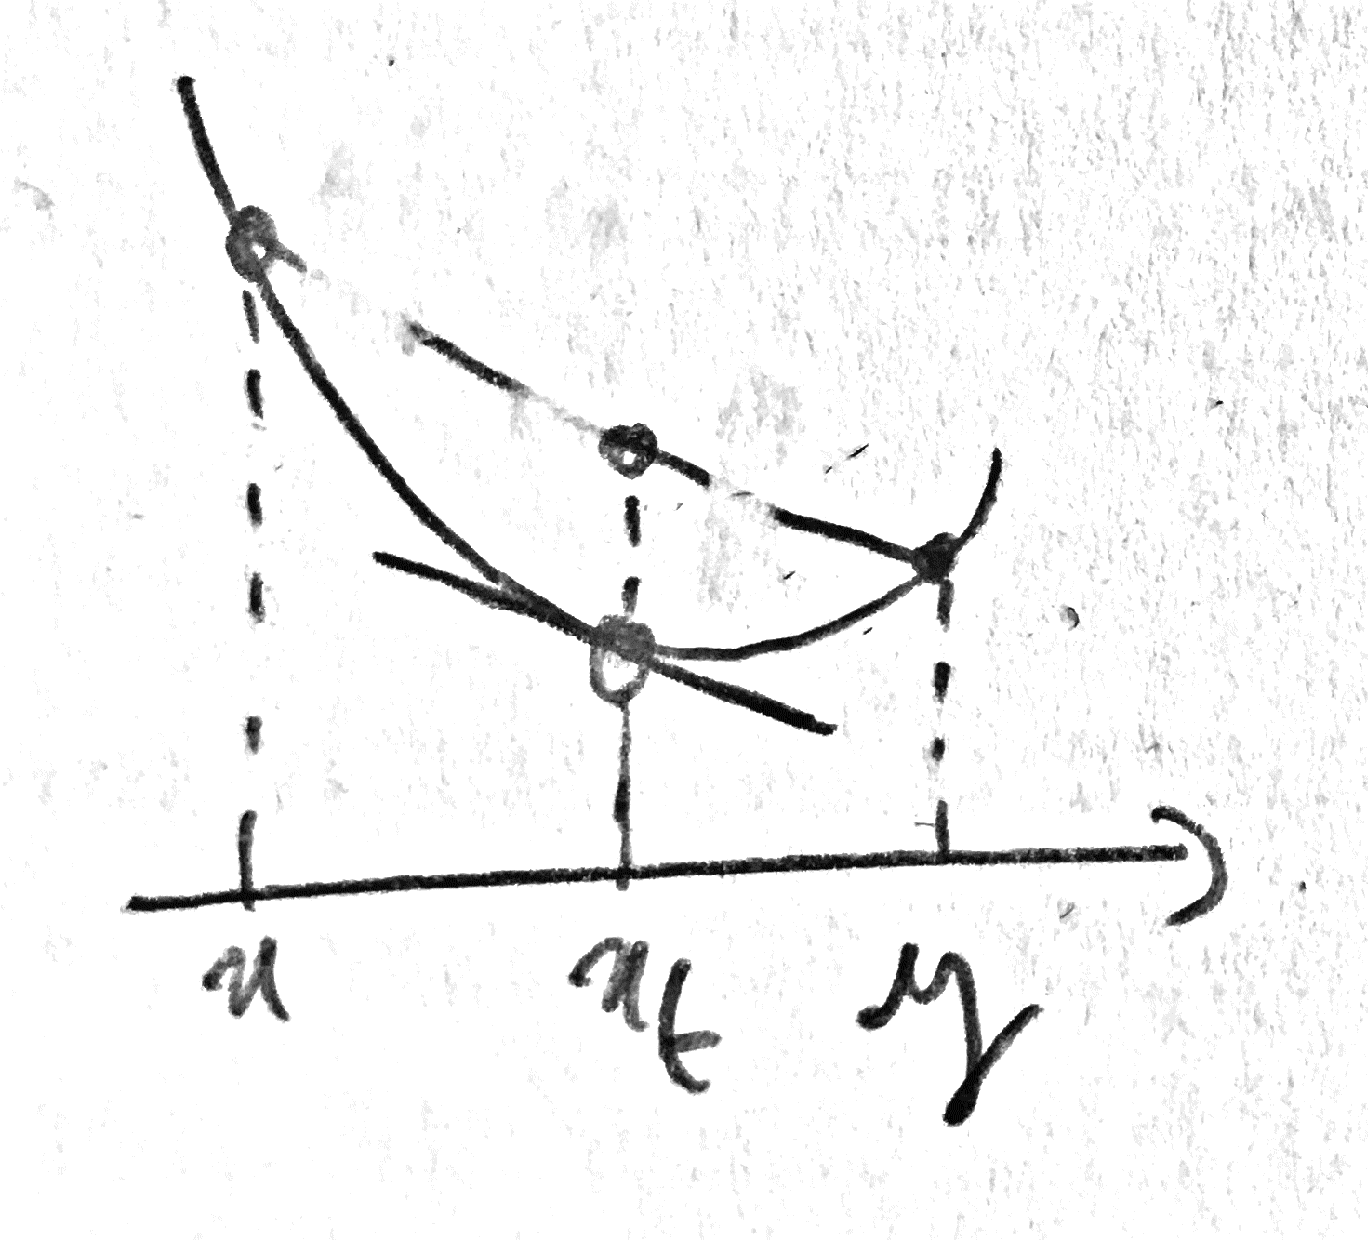
\includegraphics[width=.2\linewidth]{optim-smooth/cvx-vs-noncvx-2} &
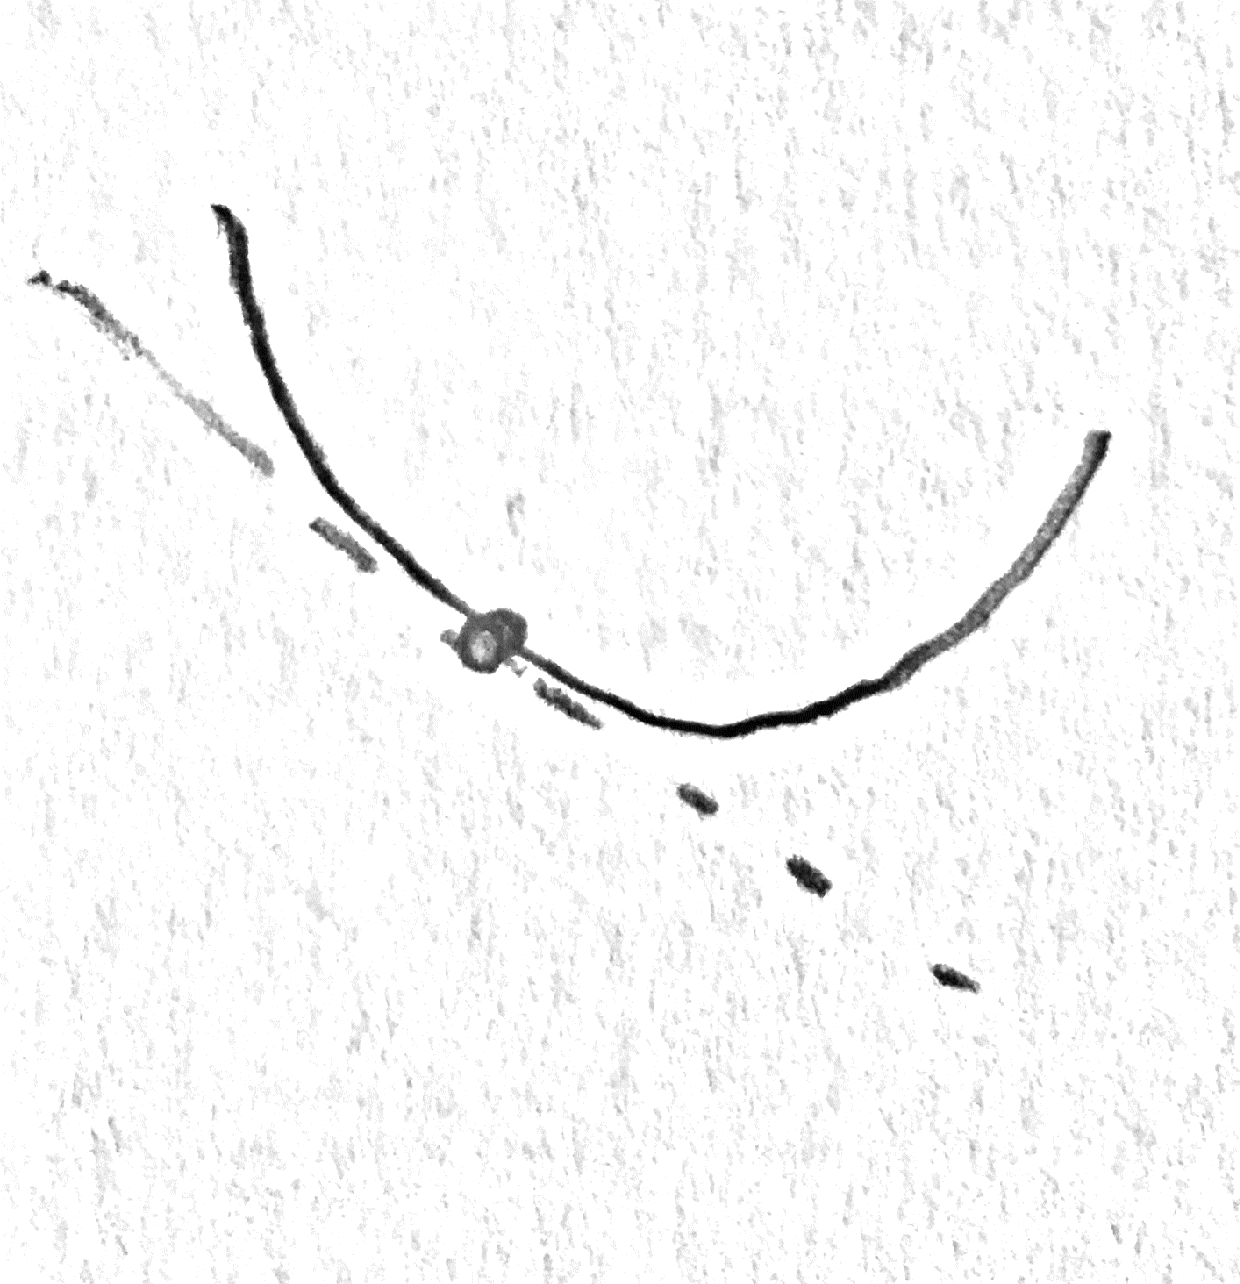
\includegraphics[width=.2\linewidth]{optim-smooth/strictly-cvx-2} &
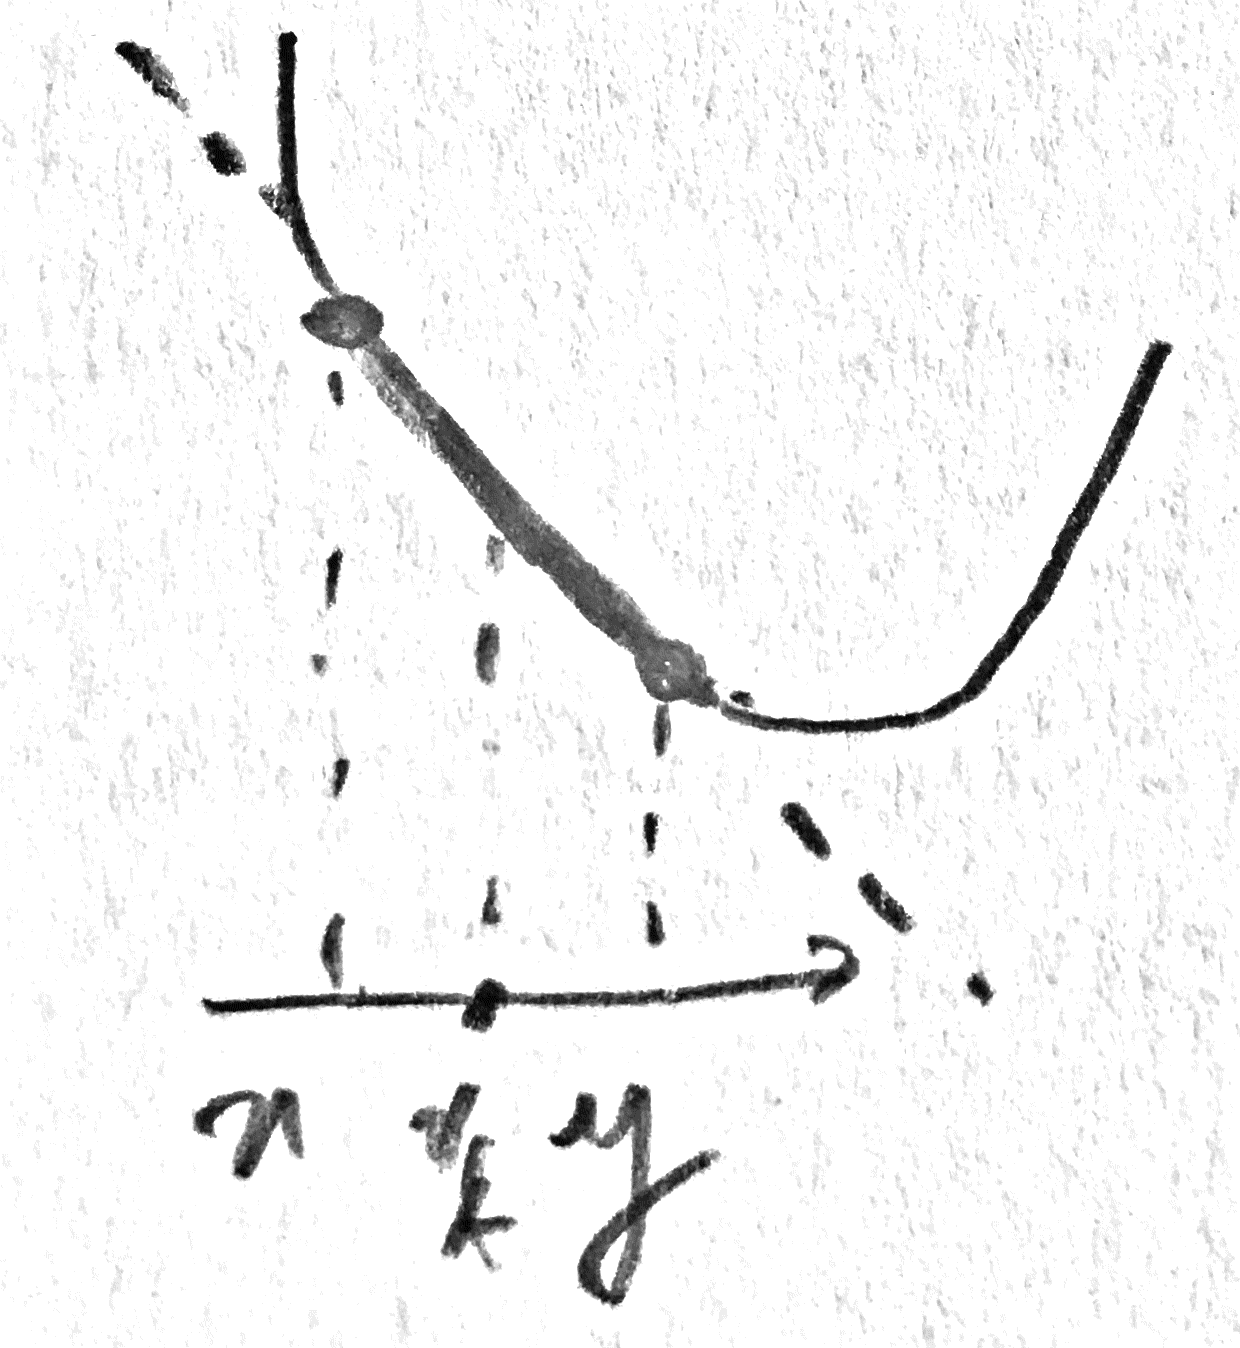
\includegraphics[width=.15\linewidth]{optim-smooth/strictly-cvx-1} 
\end{tabular}
\caption{\label{fig-cvx-vs-noncvx}
Convex vs. non-convex functions ; Strictly convex vs. non strictly convex functions.
}
\end{figure}



\begin{figure}
\centering
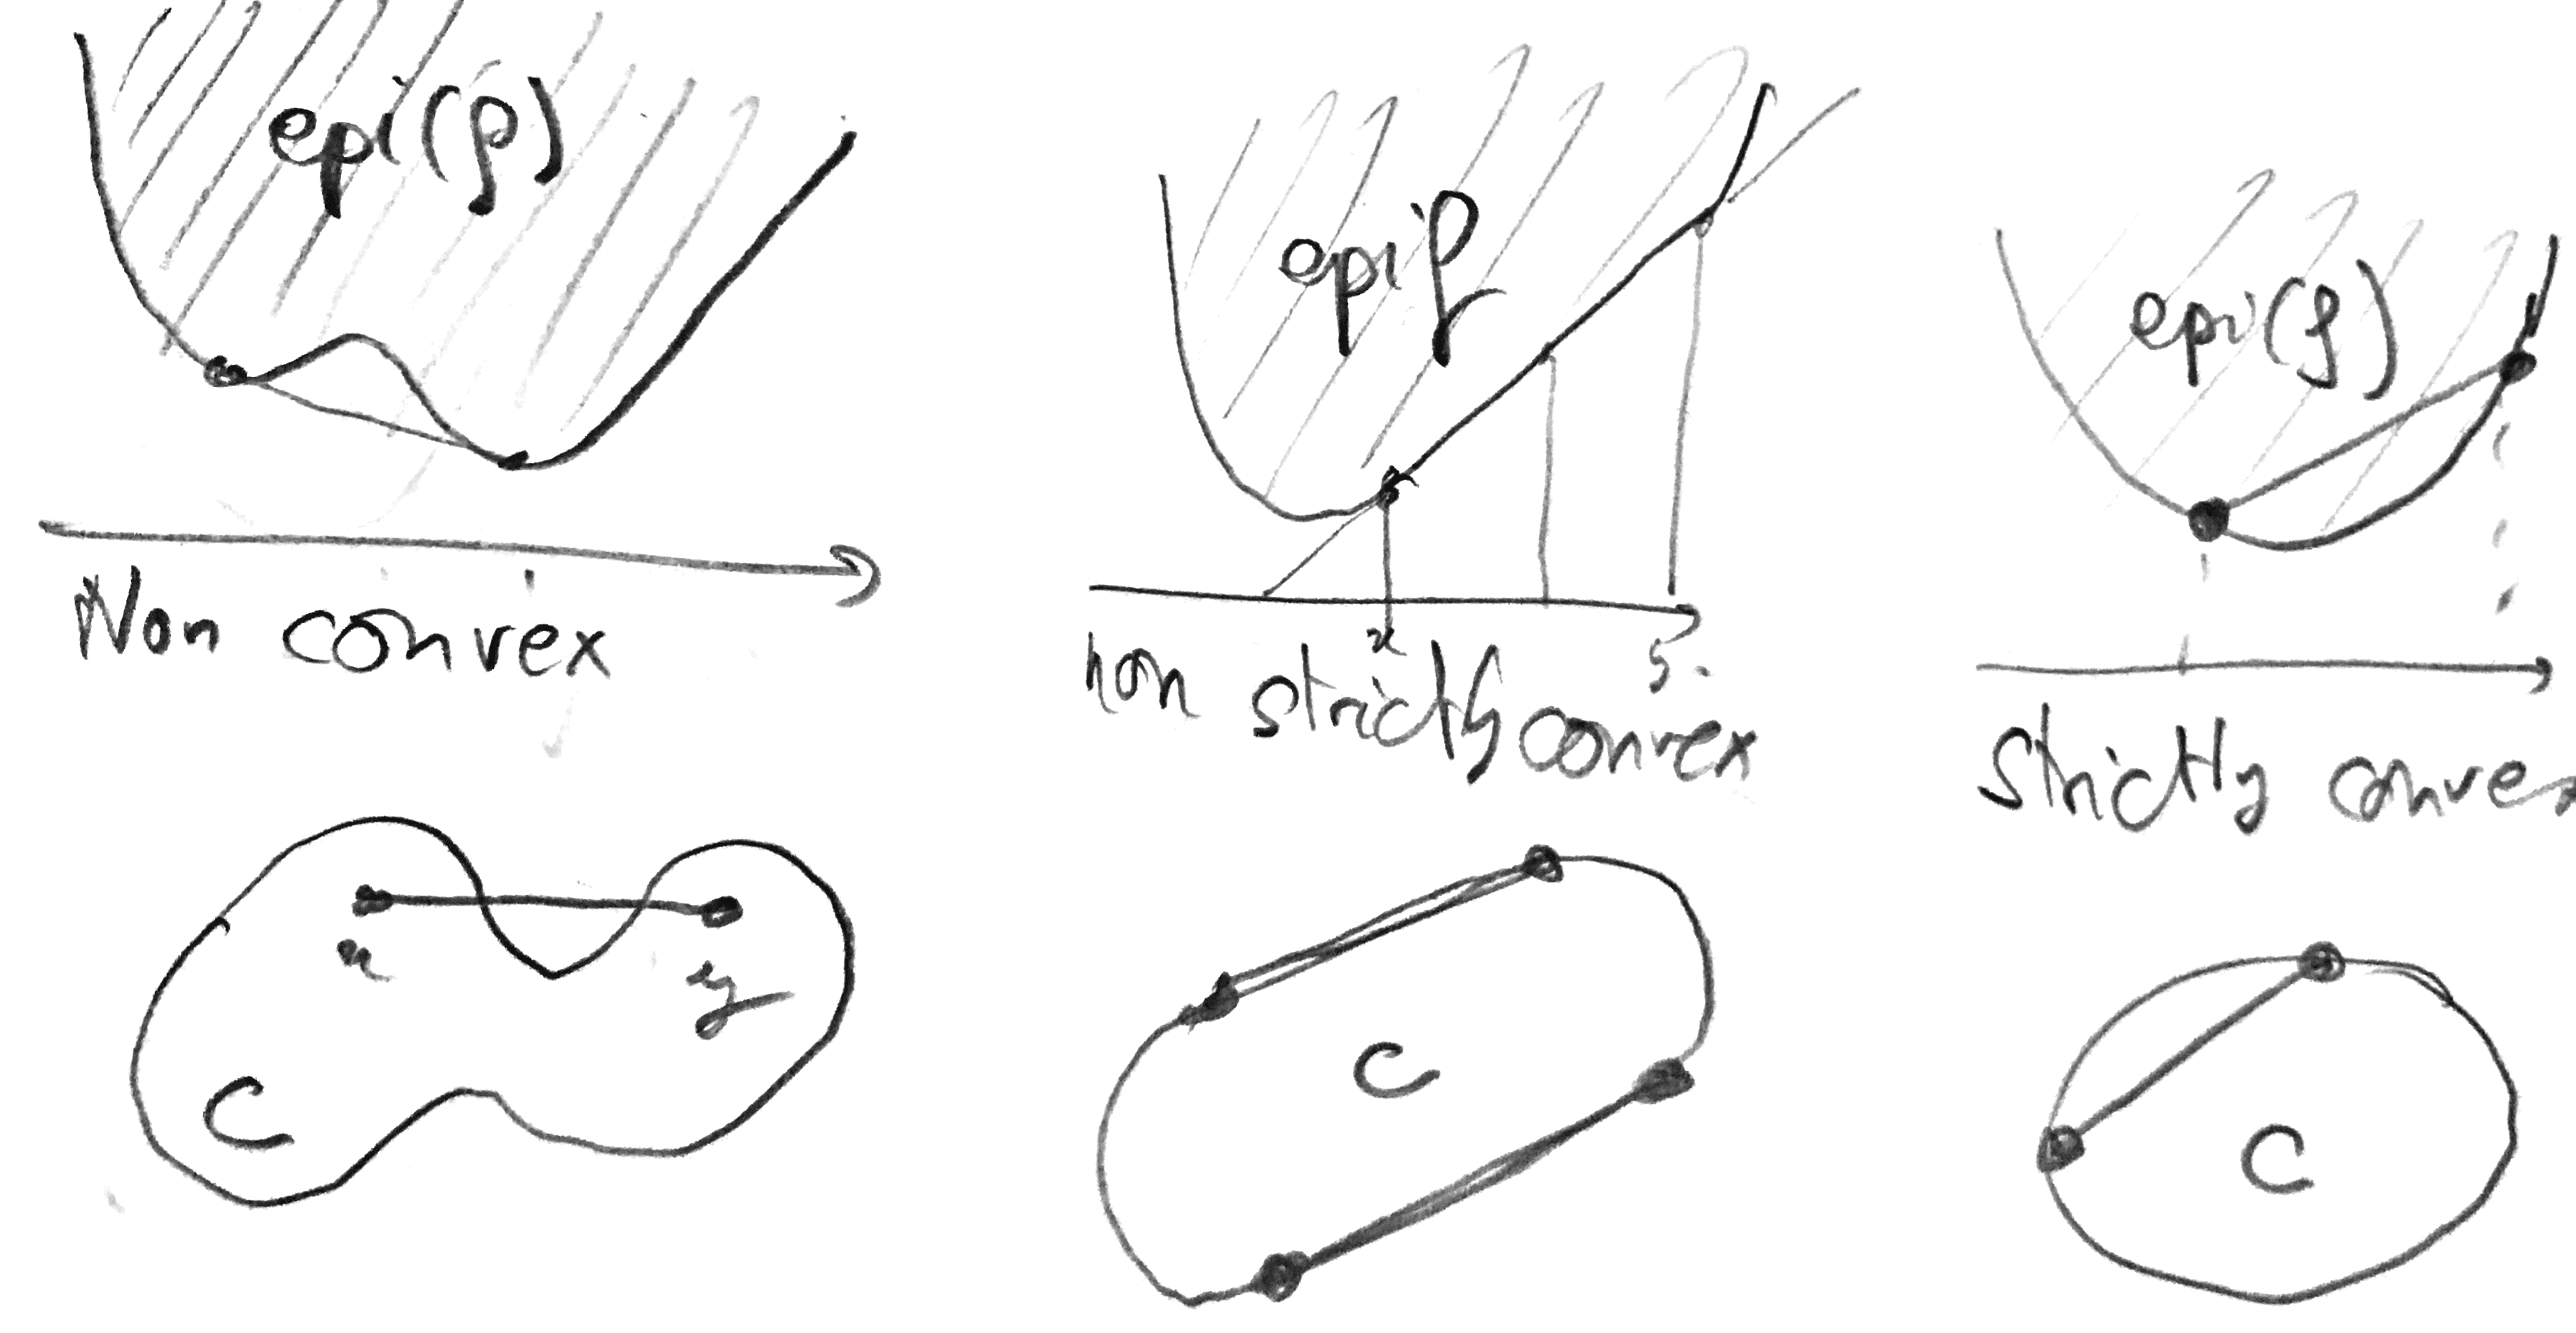
\includegraphics[width=.6\linewidth]{optim-smooth/convex-examples.png} 
\caption{\label{fig-cvx-set}
Comparison of convex functions $f : \RR^p \rightarrow \RR$ (for $p=1$) and convex sets $C \subset \RR^p$ (for $p=2$).
}
\end{figure}

%%%
\paragraph{Strict convexity.}

When $f$ is convex, one can strengthen the condition~\eqref{eq-convexity-def} and impose that the inequality is strict for $t \in ]0,1[$ (see Fig.~\ref{fig-cvx-vs-noncvx}, right), i.e.
\eql{\label{eq-strict-convexity-def}
	\foralls t \in ]0,1[, \quad
		f((1-t)x + t y) < (1-t)f(x) + t f(y).
}
In this case, if a minimum $x^\star$ exists, then it is unique.  Indeed, if $x_1^\star \neq x_2^\star$ were two different minimizer, one would have by strict convexity $f(\frac{x_1^\star+x_2^\star}{2}) < f(x_1^\star)$ which is impossible.

\begin{exmp}[Least squares]
	For the quadratic loss function $f(x)=\frac{1}{2}\norm{Ax-y}^2$, strict convexity is equivalent to $\ker(A)=\{0\}$.
	Indeed, we see later that its second derivative is $\partial^2 f(x)=A^\top A$ and that strict convexity is implied by the eigenvalues of $A^\top A$ being strictly positive. The eigenvalues of $A^\top A$ being positive, it is equivalent to $\ker(A^\top A)=\{0\}$ (no vanishing eigenvalue), and $A^\top A z = 0$ implies $\dotp{A^\top A z}{z}=\norm{Az}^2=0$ i.e. $z \in \ker(A)$.
\end{exmp}

%%%%%%%%%%%%%%%%%%%%%%%%%%%%%%%%%%%%%%%%%%%%%%%%%%%%%%%%%%%%%%%%%%%%%%%%%%%%%%%%%%
\subsection{Convex Sets}

A set $\Om \subset \RR^p$ is said to be convex if for any $(x,y) \in \Om^2$, $(1-t)x + t y \in \Om$ for $t \in [0,1]$.
%
The connexion between convex function and convex sets is that a function $f$ is convex if and only if its epigraph $\text{epi}(f) \eqdef \enscond{(x,t) \in \RR^{p+1}}{t \geq f(x)}$ is a convex set. 

\begin{rem}[Convexity of the set of minimizers]
In general, minimizers $x^\star$ might be non-unique, as shown on Figure~\ref{fig-least-square}. 
%
When $f$ is convex, the set $\argmin(f)$ of minimizers is itself a convex set. 
%
Indeed, if $x_1^\star$ and $x_2^\star$ are minimizers, so that in particular $f(x_1^\star)=f(x_2^\star)=\min(f)$, then $f( (1-t)x_1^\star + t x_2^\star ) \leq (1-t) f(x_1^\star) + t f(x_2^\star) = f(x_1^\star) = \min(f)$, so that $(1-t)x_1^\star + t x_2^\star$ is itself a minimizer. Figure~\ref{fig-cvx-set} shows convex and non-convex sets. 
\end{rem}



%%%%%%%%%%%%%%%%%%%%%%%%%%%%%%%%%%%%%%%%%%%%%%%%%%%%%%%%%%%%%%%%%%%%%%%%%%%%%%%%%%
%%%%%%%%%%%%%%%%%%%%%%%%%%%%%%%%%%%%%%%%%%%%%%%%%%%%%%%%%%%%%%%%%%%%%%%%%%%%%%%%%%
%%%%%%%%%%%%%%%%%%%%%%%%%%%%%%%%%%%%%%%%%%%%%%%%%%%%%%%%%%%%%%%%%%%%%%%%%%%%%%%%%%
\section{Derivative and gradient}

%%%%%%%%%%%%%%%%%%%%%%%%%%%%%%%%%%%%%%%%%%%%%%%%%%%%%%%%%%%%%%%%%%%%%%%%%%%%%%%%%%
\subsection{Gradient}


\wrapfSimple{optim-smooth/gradient-vector-field}
If $f$ is differentiable along each axis, we denote 
\eq{
	\nabla f(x) \eqdef \pa{\pd{f(x)}{x_1}, \ldots,\pd{f(x)}{x_p}}^\top \in \RR^p
}
the gradient vector, so that $\nabla f : \RR^p \rightarrow \RR^p$ is a vector field. Here the partial derivative (when they exits) are defined as
\eq{
	\pd{f(x)}{x_k} \eqdef \lim_{\eta \rightarrow 0} \frac{f(x+\eta \de_k)-f(x)}{\eta} 
}
where $\de_k=(0,\ldots,0,1,0,\ldots,0)^\top \in \RR^p$ is the $k^{\text{th}}$ canonical basis vector.  

Beware that $\nabla f(x)$ can exist without $f$ being differentiable. Differentiability of $f$ at each reads
\eql{\label{eq-grad-dfn}
	f(x+\epsilon) = f(x) + \dotp{\epsilon}{\nabla f(x)} + o(\norm{\epsilon}).
} 
%
Here $R(\epsilon) = o(\norm{\epsilon})$ denotes a quantity which decays faster than $\epsilon$ toward $0$, i.e. $\frac{R(\epsilon)}{\norm{\epsilon}} \rightarrow 0$ as $\epsilon \rightarrow 0$. Existence of partial derivative corresponds to $f$ being differentiable along the axes, while differentiability should hold for any converging sequence of $\epsilon\rightarrow 0$ (i.e. not along along a fixed direction). 

Also, $\nabla f(x)$ is the only vector such that the relation~\eqref{eq-grad-dfn}. This means that a possible strategy to both prove that $f$ is differentiable and to obtain a formula for $\nabla f(x)$ is to show a relation of the form 
\eq{
	f(x+\epsilon) = f(x) + \dotp{\epsilon}{g} + o(\norm{\epsilon}), 
}
in which case one necessarily has $\nabla f(x)=g$. 

The following proposition shows that convexity is equivalent to the graph of the function being above its tangents.

\begin{prop}\label{prop-above-tgt}
	If $f$ is differentiable, then
	\eq{
		f \text{ convex} 
		\quad\Leftrightarrow\quad
		\forall (x,x'), \: f(x) \geq f(x') + \dotp{\nabla f(x')}{x-x'}.
	}
\end{prop}
\begin{proof}
	One can write the convexity condition as
	\eq{
		f((1-t)x+tx') \leq (1-t) f(x) + t f(x')
		\qarrq
		\frac{ f( x + t (x'-x) ) - f(x) }{t} \leq f(x')-f(x)
	}
	hence, taking the limit $t \rightarrow 0$ one obtains
	\eq{
		\dotp{\nabla f(x)}{x'-x} \leq f(x')-f(x).
	}
	For the other implication, we apply the right condition replacing $(x,x')$ by $(x, x_t \eqdef (1-t)x+t x')$
	and $(x', (1-t)x+t x')$
	\begin{align*}
		f(x)  & \geq f(x_t) + \dotp{\nabla f(x_t)}{x-x_t} = f(x_t) - t \dotp{\nabla f(x_t)}{x-x'} \\
		f(x') & \geq f(x_t) + \dotp{\nabla f(x_t)}{x'-x_t} = f(x_t) + (1-t) \dotp{\nabla f(x_t)}{x-x'}, 
	\end{align*}
	multiplying these inequality by respectively $1-t$ and $t$, and summing them, gives
	\eq{
		(1-t)f(x)+t f(x') \geq f(x_t).
	}
\end{proof}


%%%%%%%%%%%%%%%%%%%%%%%%%%%%%%%%%%%%%%%%%%%%%%%%%%%%%%%%%%%%%%%%%%%%%%%%%%%%%%%%%%
\subsection{First Order Conditions}

The main theoretical interest (we will see later that it also have algorithmic interest) of the gradient vector is that it is a necessarily condition for optimality, as stated bellow. 

\begin{prop}\label{prop-cs-min} 
If $x^\star$ is a local minimum of the function $f$ (i.e. that $f(x^\star) \leq f(x)$ for all $x$ in some ball around $x^\star$) then 
\eq{
	\nabla f(x^\star) = 0. 
} 
\end{prop}
\begin{proof}
One has for $\epsilon$ small enough and $u$ fixed 
\eq{
	f(x^\star) \leq f(x^\star+\epsilon u) = f(x^\star) + \epsilon \dotp{\nabla f(x^\star)}{u} + o(\epsilon) 
	\qarrq
	\dotp{\nabla f(x^\star)}{u} \geq o(1)
	\qarrq
	\dotp{\nabla f(x^\star)}{u} \geq 0.
}	
So applying this for $u$ and $-u$ in the previous equation shows that $\dotp{\nabla f(x^\star)}{u}=0$ for all $u$, and hence $\nabla f(x^\star)=0$.
\end{proof}

Note that the converse is not true in general, since one might have $\nabla f(x)=0$ but $x$ is not a local mininimum. For instance $x=0$ for $f(x)=-x^2$ (here $x$ is a maximizer) or $f(x)=x^3$ (here $x$ is neither a maximizer or a minimizer, it is a saddle point), see Fig.~\ref{fig-first-order}. 
%
Note however that in practice, if $\nabla f(x^\star) = 0$ but $x$ is not a local minimum, then $x^\star$ tends to be an unstable equilibrium. Thus most often a gradient-based algorithm will converge to points with $\nabla f(x^\star) = 0$ that are local minimizers.
%
The following proposition shows that a much strong result holds if $f$ is convex.

\begin{figure}
\centering
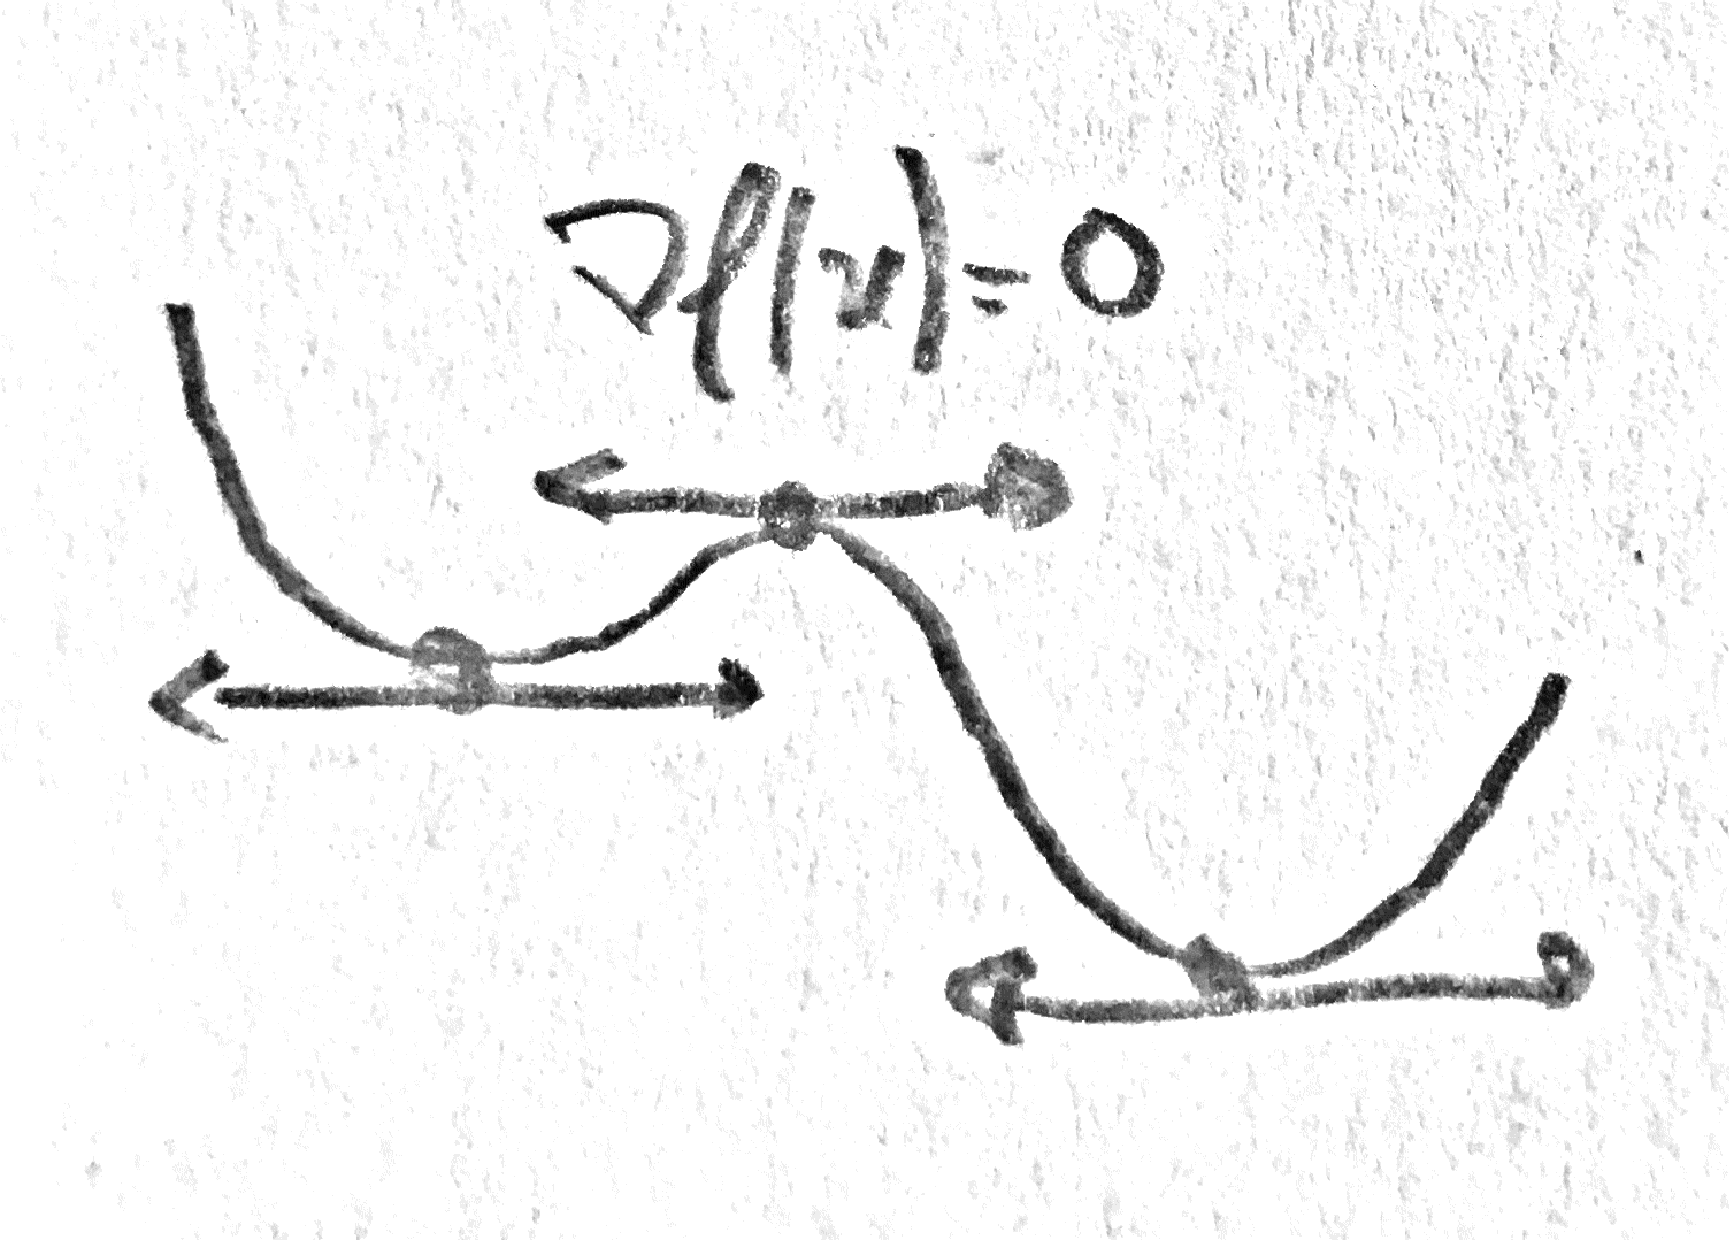
\includegraphics[width=.2\linewidth]{optim-smooth/first-order-1} \quad
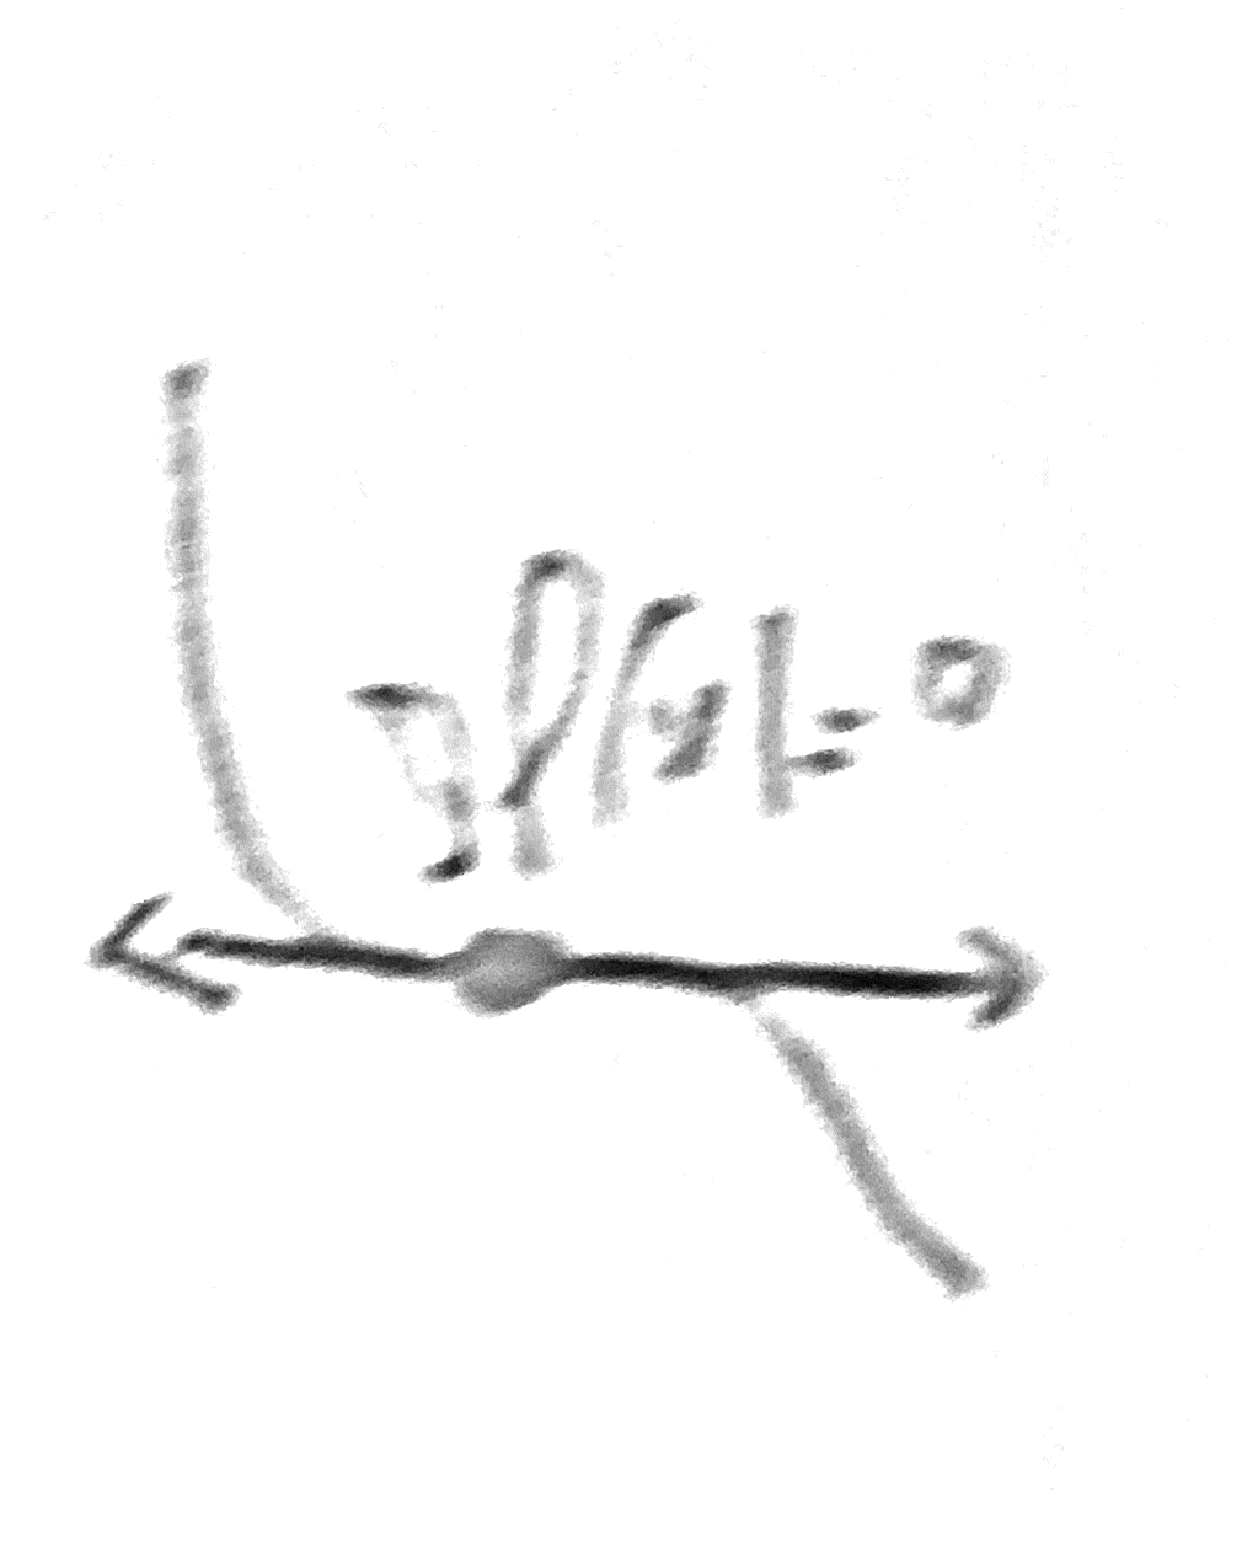
\includegraphics[width=.15\linewidth]{optim-smooth/first-order-2} \quad
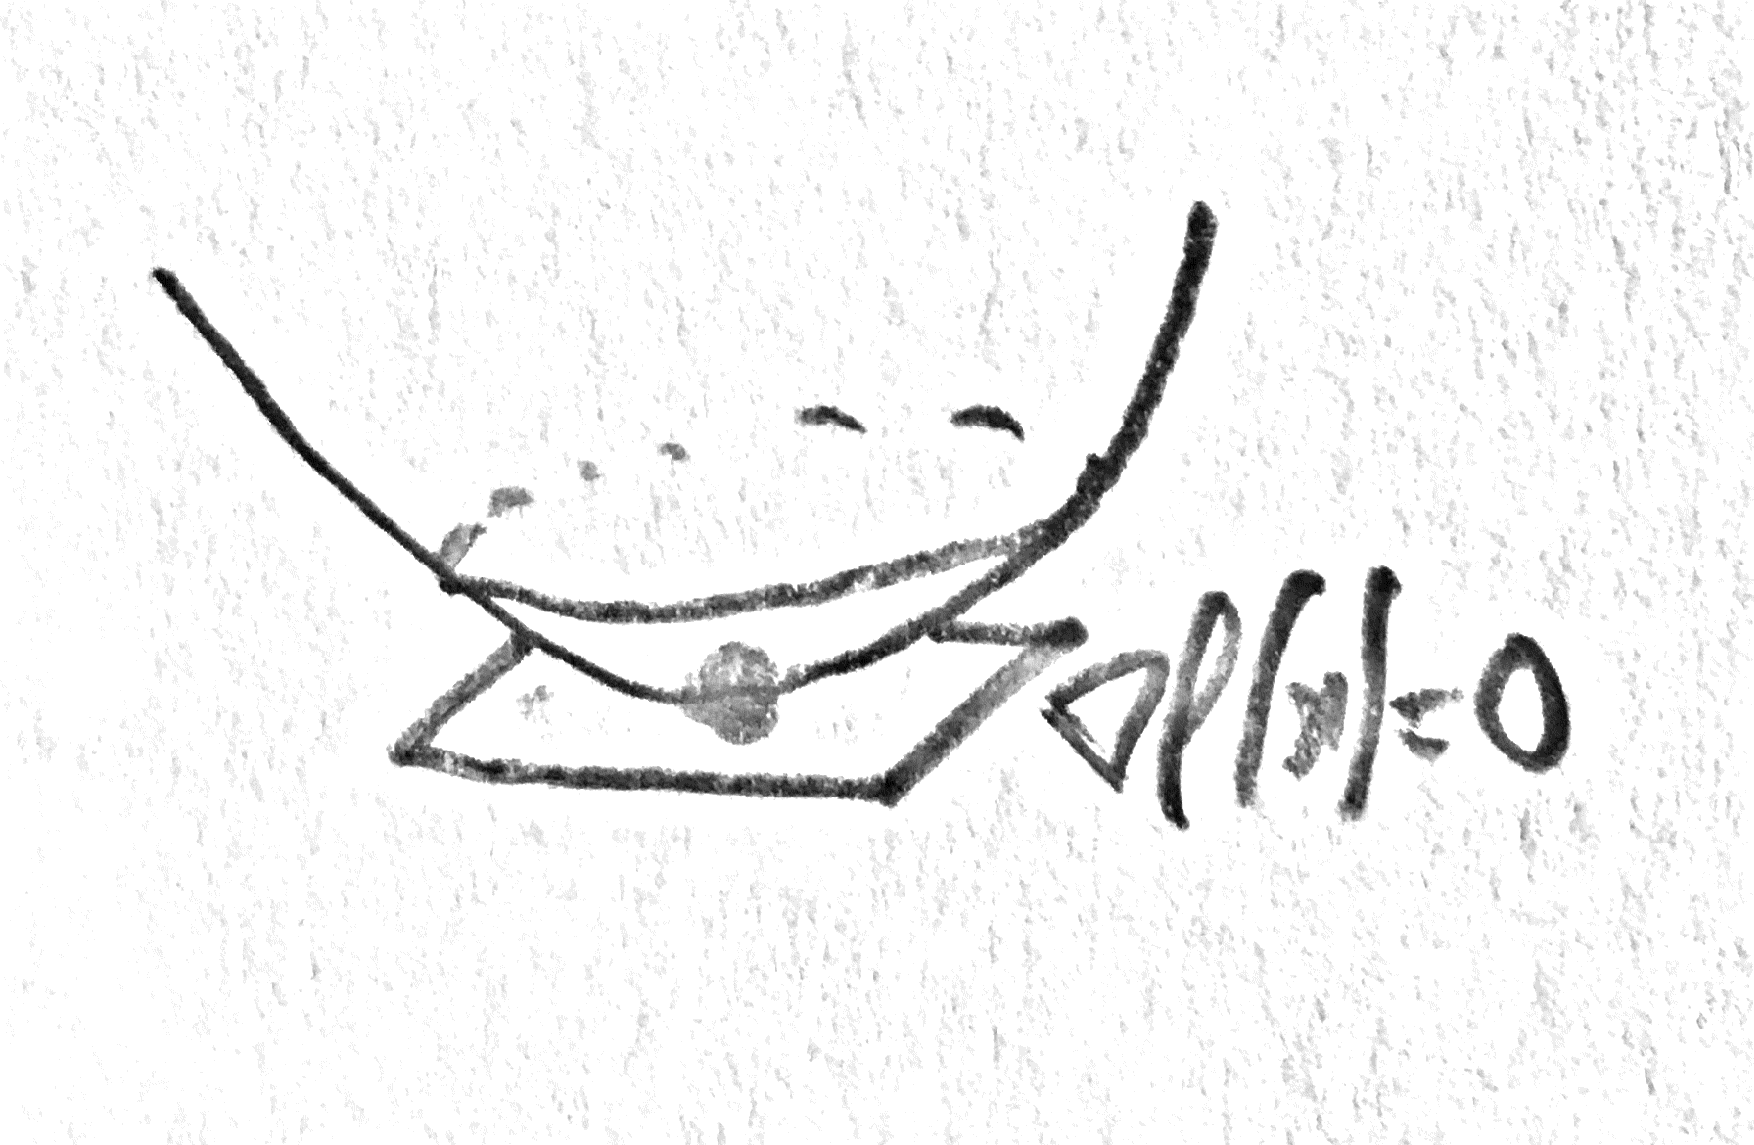
\includegraphics[width=.2\linewidth]{optim-smooth/first-order-3} 
\caption{\label{fig-first-order}
Function with local maxima/minima (left),  saddle point (middle) and global minimum (right). 
}
\end{figure}


\begin{prop} 
If $f$ is convex and $x^\star$ a local minimum, then $x^\star$ is also a global minimum.
If $f$ is differentiable and convex, 
\eq{
	x^\star \in \uargmin{x} f(x) 
	\quad\Longleftrightarrow\quad
	\nabla f(x^\star)=0.
}
\end{prop}
\begin{proof}
For any $x$, there exist $0<t<1$ small enough such that $tx + (1-t)x^\star$ is close enough to $x^\star$, and so since it is a local minimizer
\eq{
	f(x^\star) \leq f(tx + (1-t)x^\star) \leq t f(x) + (1-t) f(x^\star)
	\qarrq
	f(x^\star) \leq f(x)
}
and thus $x^\star$ is a global minimum.

For the second part, we already saw in~\eqref{prop-cs-min} the $\Leftarrow$ part. We assume that $\nabla f(x^\star)=0$. Since the graph of $x$ is above its tangent by convexity (as stated in Proposition~\ref{prop-above-tgt}), 
\eq{
	f(x) \geq f(x^\star) + \dotp{\nabla f(x^\star)}{x-x^\star} = f(x^\star).
}
\end{proof}

Thus in this case, optimizing a function is the same a solving an equation $\nabla f(x)=0$ (actually $p$ equations in $p$ unknown).
%
In most case it is impossible to solve this equation, but it often provides interesting information about solutions $x^\star$.



%%%%%%%%%%%%%%%%%%%%%%%%%%%%%%%%%%%%%%%%%%%%%%%%%%%%%%%%%%%%%%%%%%%%%%%%%%%%%%%%%%
\subsection{Least Squares}

The most important gradient formula is the one of the square loss~\eqref{eq-least-square}, which can be obtained by expanding the norm
\begin{align*}
	f(x+\epsilon) &= \frac{1}{2}\norm{Ax-y+A\epsilon}^2 = \frac{1}{2}\norm{Ax-y} + \dotp{Ax-y}{A\epsilon} + \frac{1}{2}\norm{A\epsilon}^2 \\
		&=f(x) + \dotp{\epsilon}{A^\top(Ax-y)} + o(\norm{\epsilon}).
\end{align*} 
Here, we have used the fact that $\norm{A\epsilon}^2 = o(\norm{\epsilon})$ and use the transpose matrix $A^\top$. 
%
This matrix is obtained by exchanging the rows and the columns, i.e. $A^\top = (A_{j,i})_{i=1,\ldots,n}^{j=1,\ldots,p}$, but the way it should be remember and used is that it obeys the following swapping rule of the inner product, 
\eq{
	\foralls (u,v) \in \RR^{p} \times \RR^n, \quad
	\dotp{A u}{v}_{\RR^n} = \dotp{u}{A^\top v}_{\RR^p}. 
}
Computing gradient for function involving linear operator will necessarily requires such a transposition step.
%
This computation shows that
\eql{\label{eq-grad-ls}
	\nabla f(x) = A^\top (A x - y). 
}
This implies that solutions $x^\star$ minimizing $f(x)$ satisfies the linear system $(A^\top A) x^\star = A^\top y$. 
%
If $A^\star A \in \RR^{p \times p}$ is invertible, then $f$ has a single minimizer, namely  
\eql{\label{eq-sol-leastsquare}
	x^\star = (A^\top A)^{-1} A^\top y.
}
This shows that in this case, $x^\star$ depends linearly on the data $y$, and the corresponding linear operator $(A^\top A)^{-1} A^\star$ is often called the Moore-Penrose pseudo-inverse of $A$ (which is not invertible in general, since typically $p \neq n$). 
%
The condition that $A^\top A$ is invertible is equivalent to $\ker(A)=\{0\}$, since 
\eq{
	A^\top A x = 0 \qarrq \norm{Ax}^2 = \dotp{A^\top A x}{x} = 0 \qarrq A x= 0.
}
In particular, if $n<p$ (under-determined regime, there is too much parameter or too few data) this can never holds. If $n \geq p$ and the features $x_i$ are ``random'' then $\ker(A)=\{0\}$ with probability one. In this overdetermined situation $n \geq p$,  $\ker(A)=\{0\}$ only holds if the features $\{a_i\}_{i=1}^n$ spans a linear space $\Im(A^\top)$ of dimension strictly smaller than the ambient dimension $p$.
 
%%%%%%%%%%%%%%%%%%%%%%%%%%%%%%%%%%%%%%%%%%%%%%%%%%%%%%%%%%%%%%%%%%%%%%%%%%%%%%%%%%
\subsection{Link with PCA}

Let us assume the $(a_i)_{i=1}^n$ are centered, i.e. $\sum_i a_i=0$. If this is not the case, one needs to replace
 $a_i$ by $a_i - m$ where $m \eqdef \frac{1}{n}\sum_{i=1}^n a_i \in \RR^p$ is the empirical mean. In this case, $\frac{C}{n} = A^\top A/n \in \RR^{p \times p}$ is the empirical covariance of the point cloud $(a_i)_i$, it encodes the covariances between the coordinates of the points. Denoting $a_i = (a_{i,1},\ldots,a_{i,p})^\top \in \RR^p$ (so that $A=(a_{i,j})_{i,j}$) the coordinates, one has
 \eq{
 	\foralls (k,\ell) \in \{1,\ldots,p\}^2, \quad
 	\frac{C_{k,\ell}}{n} = \frac{1}{n} \sum_{i=1}^n a_{i,k} a_{i,\ell}. 
 }
 In particular, $C_{k,k}/n$ is the variance along the axis $k$. More generally, for any unit vector $u \in \RR^p$, $\dotp{C u}{u}/n \geq 0$ is the variance along the axis $u$.
 
For instance, in dimension $p=2$, 
\eq{
	\frac{C}{n} = 
	\frac{1}{n}
	\begin{pmatrix}
		 \sum_{i=1}^n a_{i,1}^2 & \sum_{i=1}^n a_{i,1} a_{i,2} \\
		\sum_{i=1}^n a_{i,1}a_{i,2} & \sum_{i=1}^n a_{i,2}^2
	\end{pmatrix}.
}

Since $C$ is a symmetric, it diagonalizes in an ortho-basis $U=(u_1,\ldots,u_p) \in \RR^{p \times p}$. Here, the vectors $u_k \in \RR^p$ are stored in the columns of the matrix $U$. The diagonalization means that there exist scalars (the eigenvalues) $(\la_1,\ldots,\la_p)$ so that $(\frac{1}{n} C) u_k = \la_k u_k$. Since the matrix is orthogononal, $UU^\top = U^\top U = \Id_p$, and equivalently $U^{-1}=U^\top$. The diagonalization property can be conveniently written as $\frac{1}{n} C=U \diag(\la_k) U^\top$. One can thus re-write the covariance quadratic form in the basis $U$ as being a separable sum of $p$ squares
\eql{\label{eq-pca-decomp}
	\frac{1}{n}  \dotp{Cx}{x} = \dotp{U \diag(\la_k) U^\top x}{x}
	= \dotp{\diag(\la_k) (U^\top x)}{(U^\top x)}
	= \sum_{k=1}^p \la_k \dotp{x}{u_k}^2.
} 
Here $( U^\top x )_k = \dotp{x}{u_k}$ is the coordinate $k$ of $x$ in the basis $U$. Since $\dotp{Cx}{x}=\norm{Ax}^2$, this shows that all the eigenvalues $\la_k \geq 0$ are positive. 

\begin{figure}
\centering
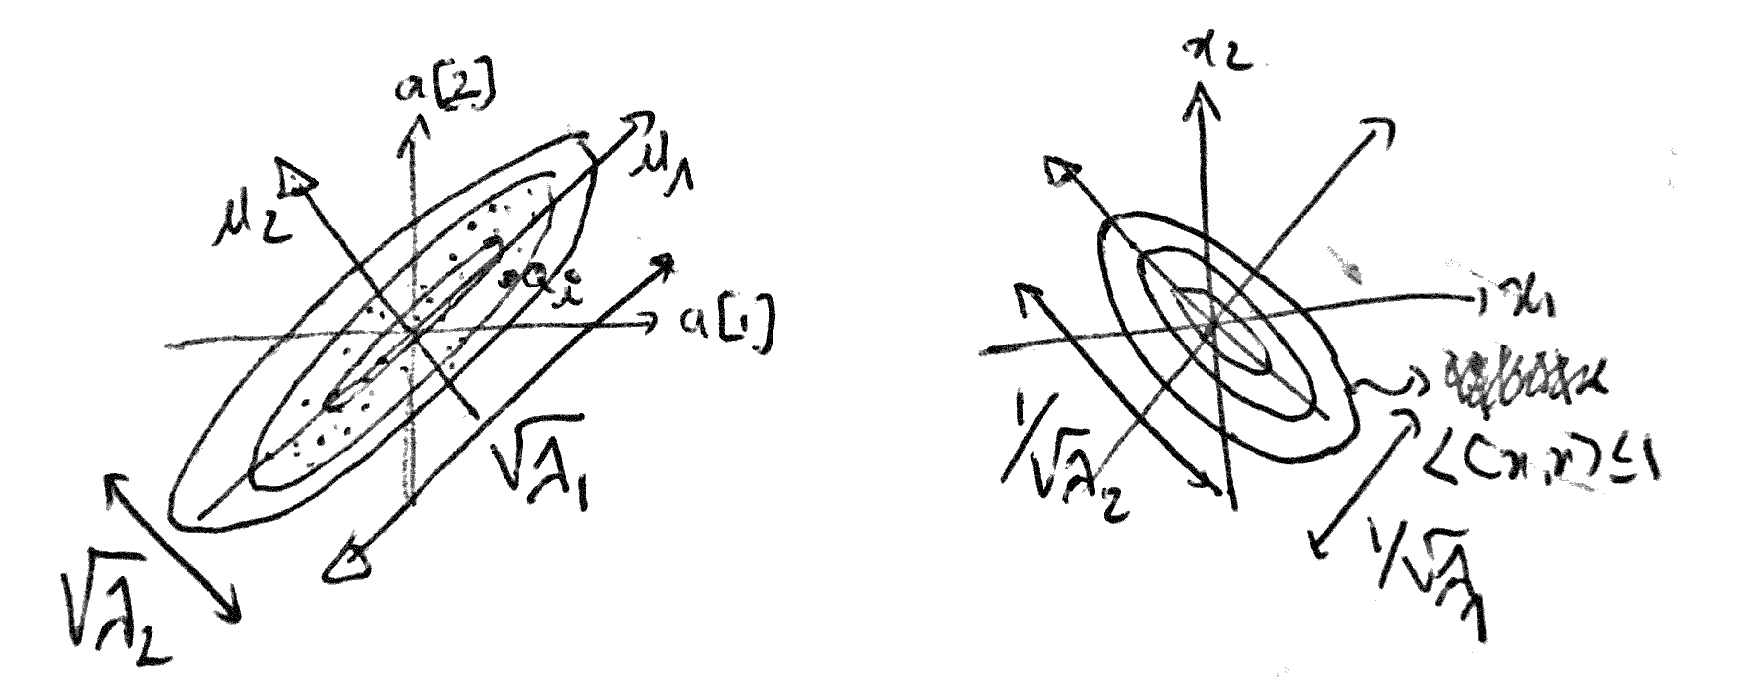
\includegraphics[width=.5\linewidth]{optim-smooth/link-pca}
\caption{\label{fig-link-pca}
Left: point clouds $(a_i)_i$ with associated PCA directions, right: quadratic part of $f(x)$.
}
\end{figure}

If one assumes that the eigenvalues are ordered $\la_1 \geq \la_2 \geq \ldots \geq \la_p$, then projecting the points $a_i$ on the first $m$ eigenvectors can be shown to be in some sense the best linear dimensionality reduction possible (see next paragraph), and it is called Principal Component Analysis (PCA). It is useful to perform compression or dimensionality reduction, but in practice, it is mostly used for data visualization in 2-D ($m=2$) and 3-D ($m=3$).

The matrix $C/n$ encodes the covariance, so one can approximate the point cloud by an ellipsoid whose main axes are the $(u_k)_k$ and the width along each axis is $\propto \sqrt{\la_k}$ (the standard deviations). 
%
If the data are approximately drawn from a Gaussian distribution, whose density is proportional to $\exp(\frac{-1}{2}\dotp{C^{-1}a}{a})$, then the fit is good.
%
This should be contrasted with the shape of quadratic part $\frac{1}{2}\dotp{Cx}{x}$ of $f(x)$, since the ellipsoid $\enscond{x}{\frac{1}{n}\dotp{Cx}{x} \leq 1}$ has the same main axes, but the widths are the inverse $1/\sqrt{\la_k}$. 
%
Figure~\ref{fig-link-pca} shows this in dimension $p=2$.



%%%%%%%%%%%%%%%%%%%%%%%%%%%%%%%%%%%%%%%%%%%%%%%%%%%%%%%%%%%%%%%%%%%%%%%%%%%%%%%%%%
\subsection{Classification}

We can do a similar computation for the gradient of the classification loss~\eqref{eq-classif}. Assuming that $L$ is differentiable, and using the Taylor expansion~\eqref{eq-grad-dfn} at point $-\diag(y) Ax$, one has 
\begin{align*}
	f(x+\epsilon) &= L( -\diag(y) Ax -\diag(y)  A\epsilon) \\
	&= L(-\diag(y) Ax) + \dotp{\nabla L( -\diag(y) Ax)}{ -\diag(y)  A\epsilon } + o(\norm{\diag(y)  A\epsilon}).
\end{align*} 
Using the fact that $o(\norm{\diag(y)  A\epsilon}) = o(\norm{\epsilon})$, one obtains
\begin{align*}
	f(x+\epsilon) &= f(x) + \dotp{\nabla L( -\diag(y) Ax)}{-\diag(y)  A\epsilon} + o(\norm{\epsilon}) \\
		 &=  f(x) + \dotp{-A^\top \diag(y) \nabla L( -\diag(y) Ax)}{\epsilon} + o(\norm{\epsilon}), 
\end{align*} 	
where we have used the fact that $(AB)^\top = B^\top A^\top$ and that $\diag(y)^\top=\diag(y)$. This shows that
\eq{
	\nabla f(x) = -A^\top \diag(y) \nabla L( -\diag(y) Ax). 
}
Since $L(z) = \sum_i \ell(z_i)$, one has $\nabla L(z) = (\ell'(z_i))_{i=1}^n$. For instance, for the logistic classification method, $\ell(u) = \log(1+\exp(u))$ so that $\ell'(u) = \frac{e^u}{1+e^u} \in [0,1]$ (which can be interpreted as a probability of predicting $+1$).


%%%%%%%%%%%%%%%%%%%%%%%%%%%%%%%%%%%%%%%%%%%%%%%%%%%%%%%%%%%%%%%%%%%%%%%%%%%%%%%%%%
\subsection{Chain Rule}

One can formalize the previous computation, if $f(x) = g(Bx)$ with $B \in \RR^{q \times p}$ and $g : \RR^q \rightarrow \RR$, then
\eq{
	f(x+\epsilon) = g(Bx + B\epsilon) = g(Bx) + \dotp{\nabla g(Bx)}{B \epsilon} + o(\norm{B \epsilon})
	= f(x) + \dotp{\epsilon}{B^\top \nabla g(Bx)} + o(\norm{\epsilon}), 
}
which shows that 
\eql{\label{eq-grad-composition-linear}
	\nabla ( g \circ B ) = B^\top \circ \nabla g \circ B
}
where ``$\circ$'' denotes the composition of functions.

To generalize this to composition of possibly non-linear functions, one needs to use the notion of differential. For a function $F : \RR^p \rightarrow \RR^q$, its differentiable at $x$ is a linear operator $\partial F(x) : \RR^{p} \rightarrow \RR^q$, i.e. it can be represented as a matrix (still denoted $\partial F(x)$) $\partial F(x) \in \RR^{q \times p}$.
%
The entries of this matrix are the partial differential, denoting $F(x)=(F_1(x), \ldots, F_q(x))$, 
\eq{
	\foralls (i,j) \in \{1,\ldots,q\} \times \{1,\ldots,p\}, \quad
	[ \partial F(x) ]_{i,j} \eqdef \frac{\partial F_i(x)}{\partial x_j}.
}
The function $F$ is then said to be differentiable at $x$ if and only if one has the following Taylor expansion 
\eql{\label{eq-differential-defn}
	F(x+\epsilon) = F(x) + [\partial F(x)](\epsilon) + o(\norm{\epsilon}).
}
where $[\partial F(x)](\epsilon)$ is the matrix-vector multiplication. As for the definition of the gradient, this matrix is the only one that satisfies this expansion, so it can be used as a way to compute this differential in practice.

For the special case $q=1$, i.e. if $f : \RR^p \rightarrow \RR$, then the differential $\partial f(x) \in \RR^{1 \times p}$ and the gradient $\nabla f(x) \in \RR^{p \times 1}$ are linked by equating the Taylor expansions~\eqref{eq-differential-defn} and~\eqref{eq-grad-dfn}
\eq{
	\foralls \epsilon \in \RR^p, \quad
	[\partial f(x)](\epsilon) = \dotp{\nabla f(x)}{\epsilon}	
	\quad\Leftrightarrow\quad
	[\partial f(x)](\epsilon) = \nabla f(x)^\top. 
}

The differential satisfies the following chain rule 
\eq{
	\partial( G \circ H)(x) = [\partial G(H(x))] \times [\partial H(x)] 
}
where ``$\times$'' is the matrix product. For instance, if $H : \RR^p \rightarrow \RR^q$ and $G = g : \RR^q \mapsto \RR$, then $f = g \circ H : \RR^p \rightarrow \RR$ and one can compute its gradient as follow
\eq{
	\nabla f(x) = (\partial f(x))^\top = \pa{ [\partial g(H(x))] \times [\partial H(x)] }^\top
	= [\partial H(x)]^\top \times [\partial g(H(x))]^\top
	= [\partial H(x)]^\top \times \nabla g(H(x)).
}
When $H(x)=Bx$ is linear, one recovers formula~\eqref{eq-grad-composition-linear}.


%%%%%%%%%%%%%%%%%%%%%%%%%%%%%%%%%%%%%%%%%%%%%%%%%%%%%%%%%%%%%%%%%%%%%%%%%%%%%%%%%%
%%%%%%%%%%%%%%%%%%%%%%%%%%%%%%%%%%%%%%%%%%%%%%%%%%%%%%%%%%%%%%%%%%%%%%%%%%%%%%%%%%
%%%%%%%%%%%%%%%%%%%%%%%%%%%%%%%%%%%%%%%%%%%%%%%%%%%%%%%%%%%%%%%%%%%%%%%%%%%%%%%%%%
\section{Gradient Descent Algorithm}
\label{sec-grad-desc-basic}


%%%%%%%%%%%%%%%%%%%%%%%%%%%%%%%%%%%%%%%%%%%%%%%%%%%%%%%%%%%%%%%%%%%%%%%%%%%%%%%%%%
\subsection{Steepest Descent Direction}

The Taylor expansion~\eqref{eq-grad-dfn} computes an affine approximation of the function $f$ near $x$, since it can be written as
\eq{
	f(z) = T_x(z) + o(\norm{x-z})
	\qwhereq
	T_x(z) \eqdef f(x) + \dotp{\nabla f(x)}{z-x}, 
}
see Fig.~\ref{fig-expansion-taylor}. First order methods operate by locally replacing $f$ by $T_x$.


\begin{figure}
\centering
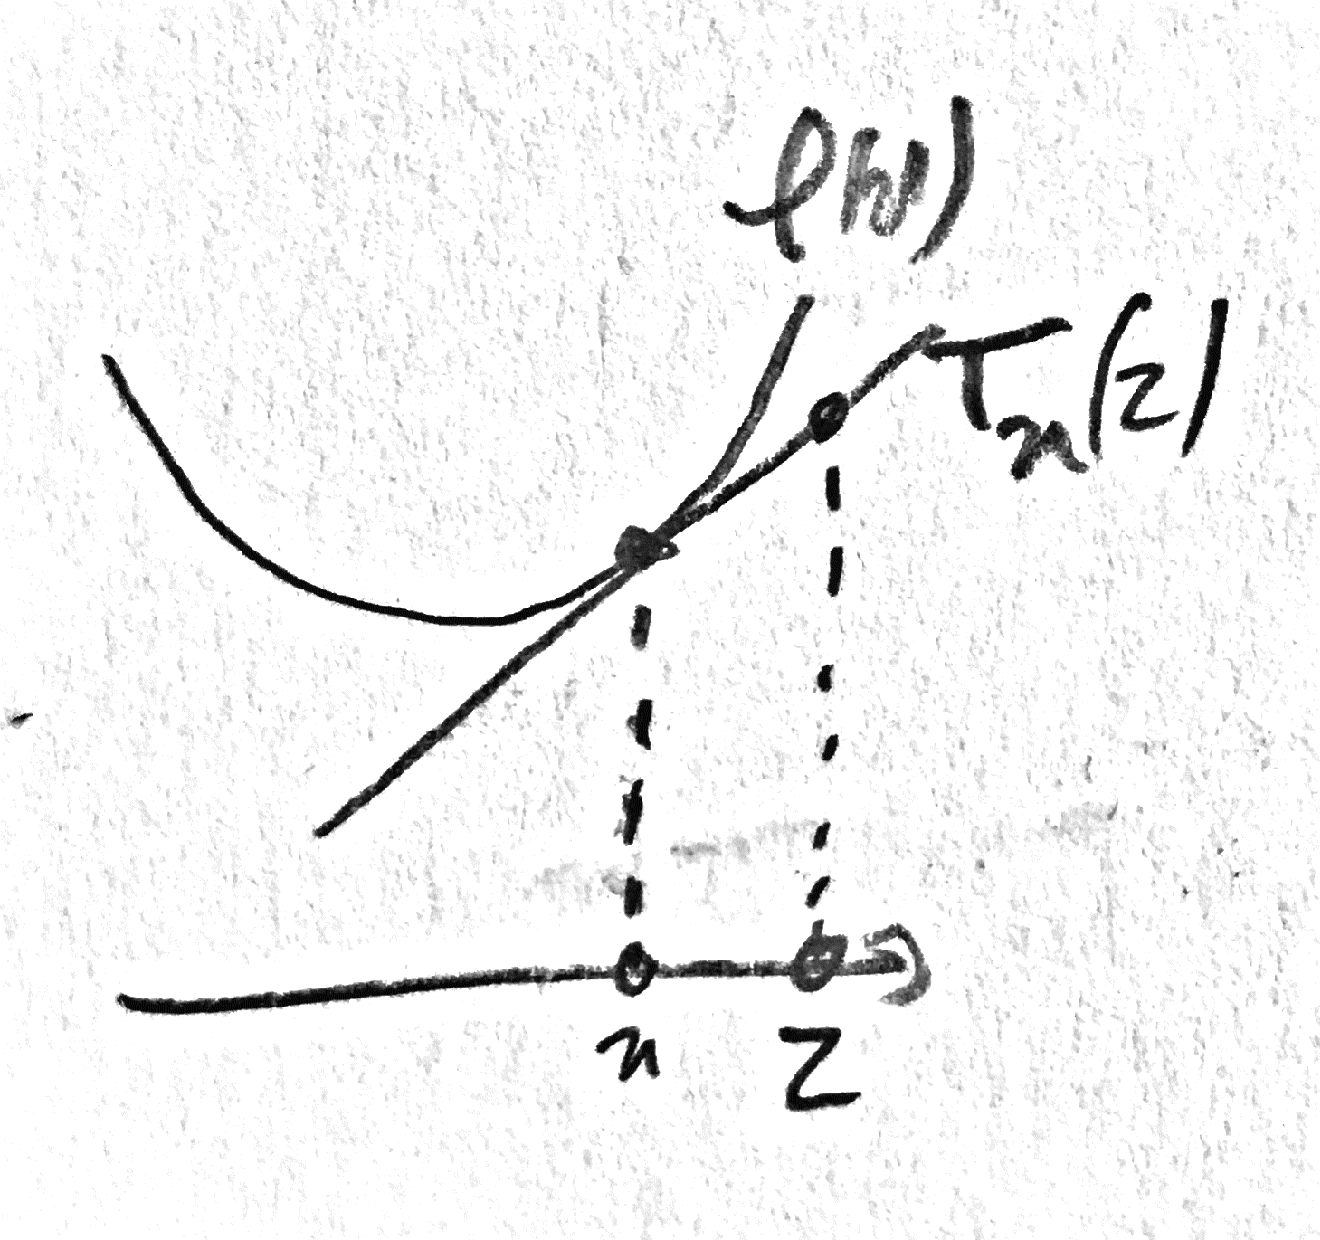
\includegraphics[width=.2\linewidth]{optim-smooth/taylor-exp-1} \quad
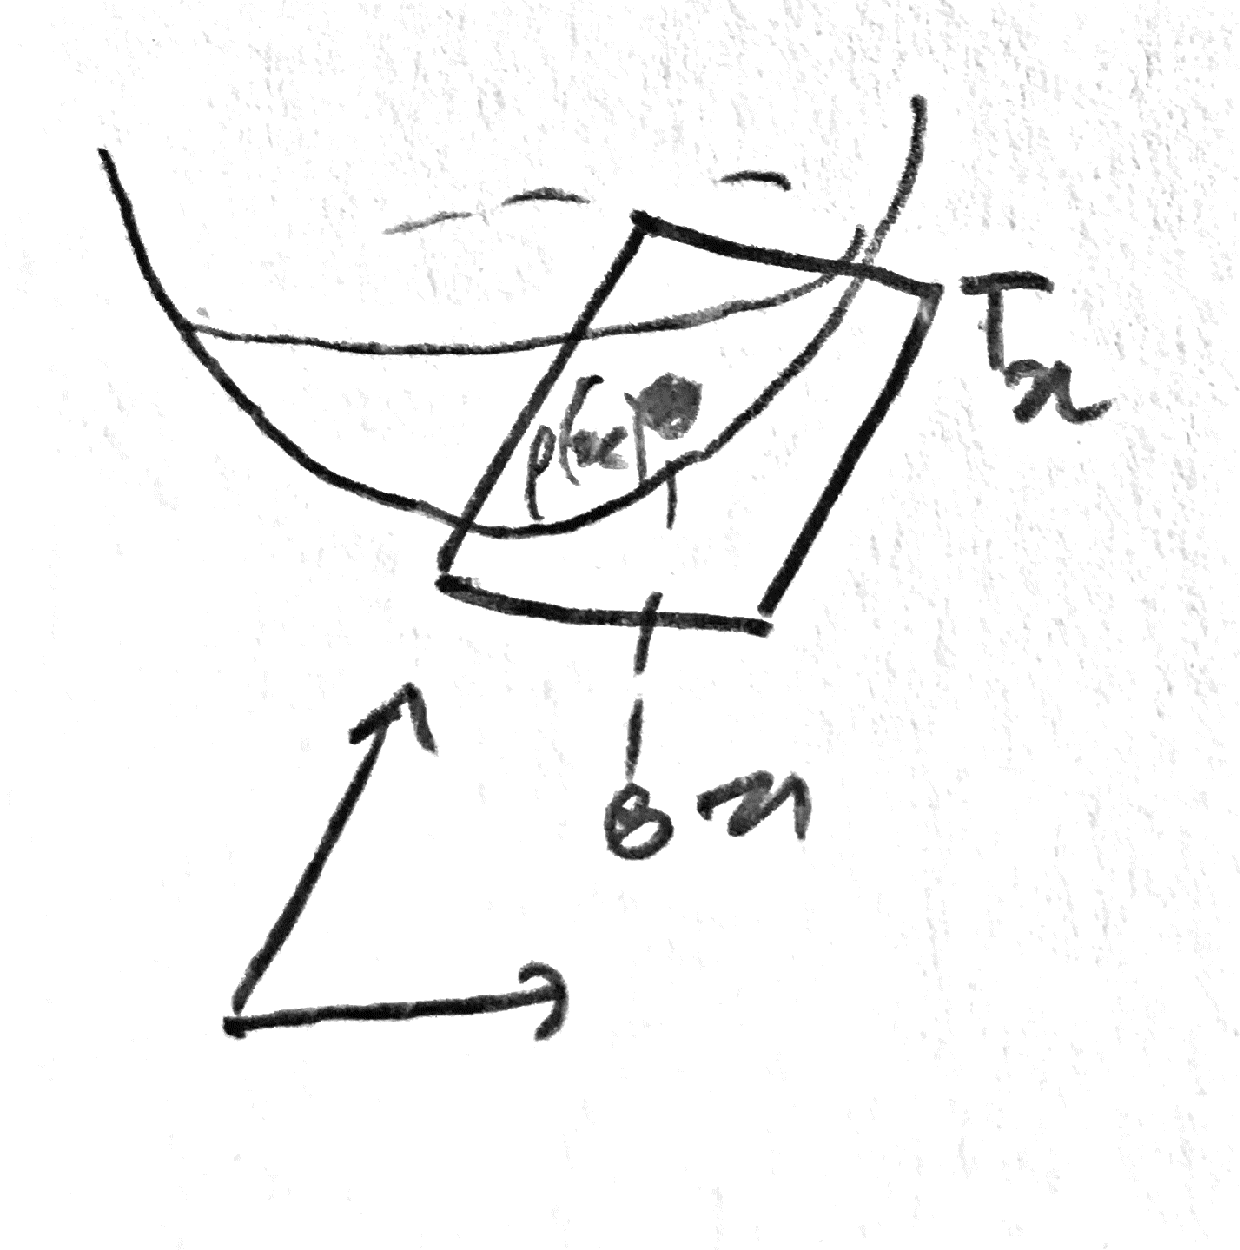
\includegraphics[width=.18\linewidth]{optim-smooth/taylor-exp-2} \quad
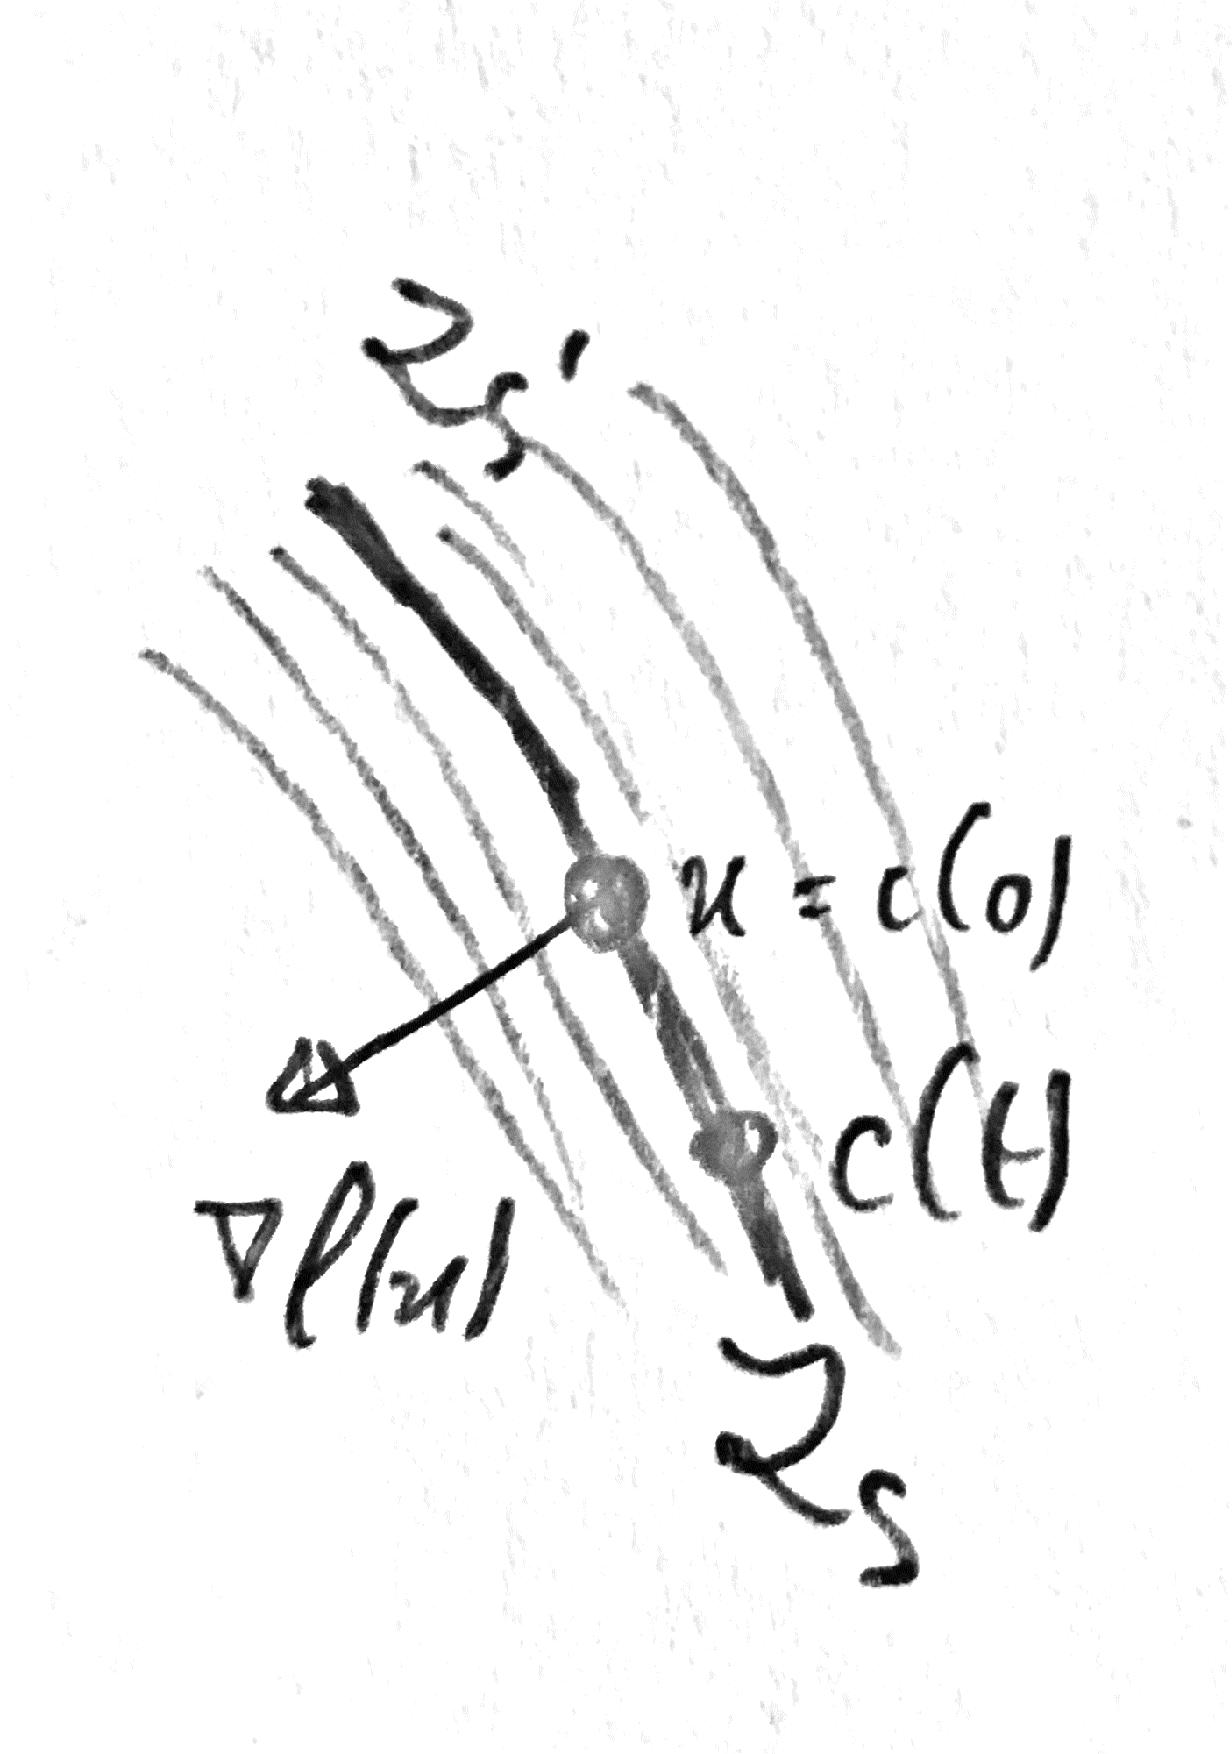
\includegraphics[width=.18\linewidth]{optim-smooth/level-sets-1} \quad
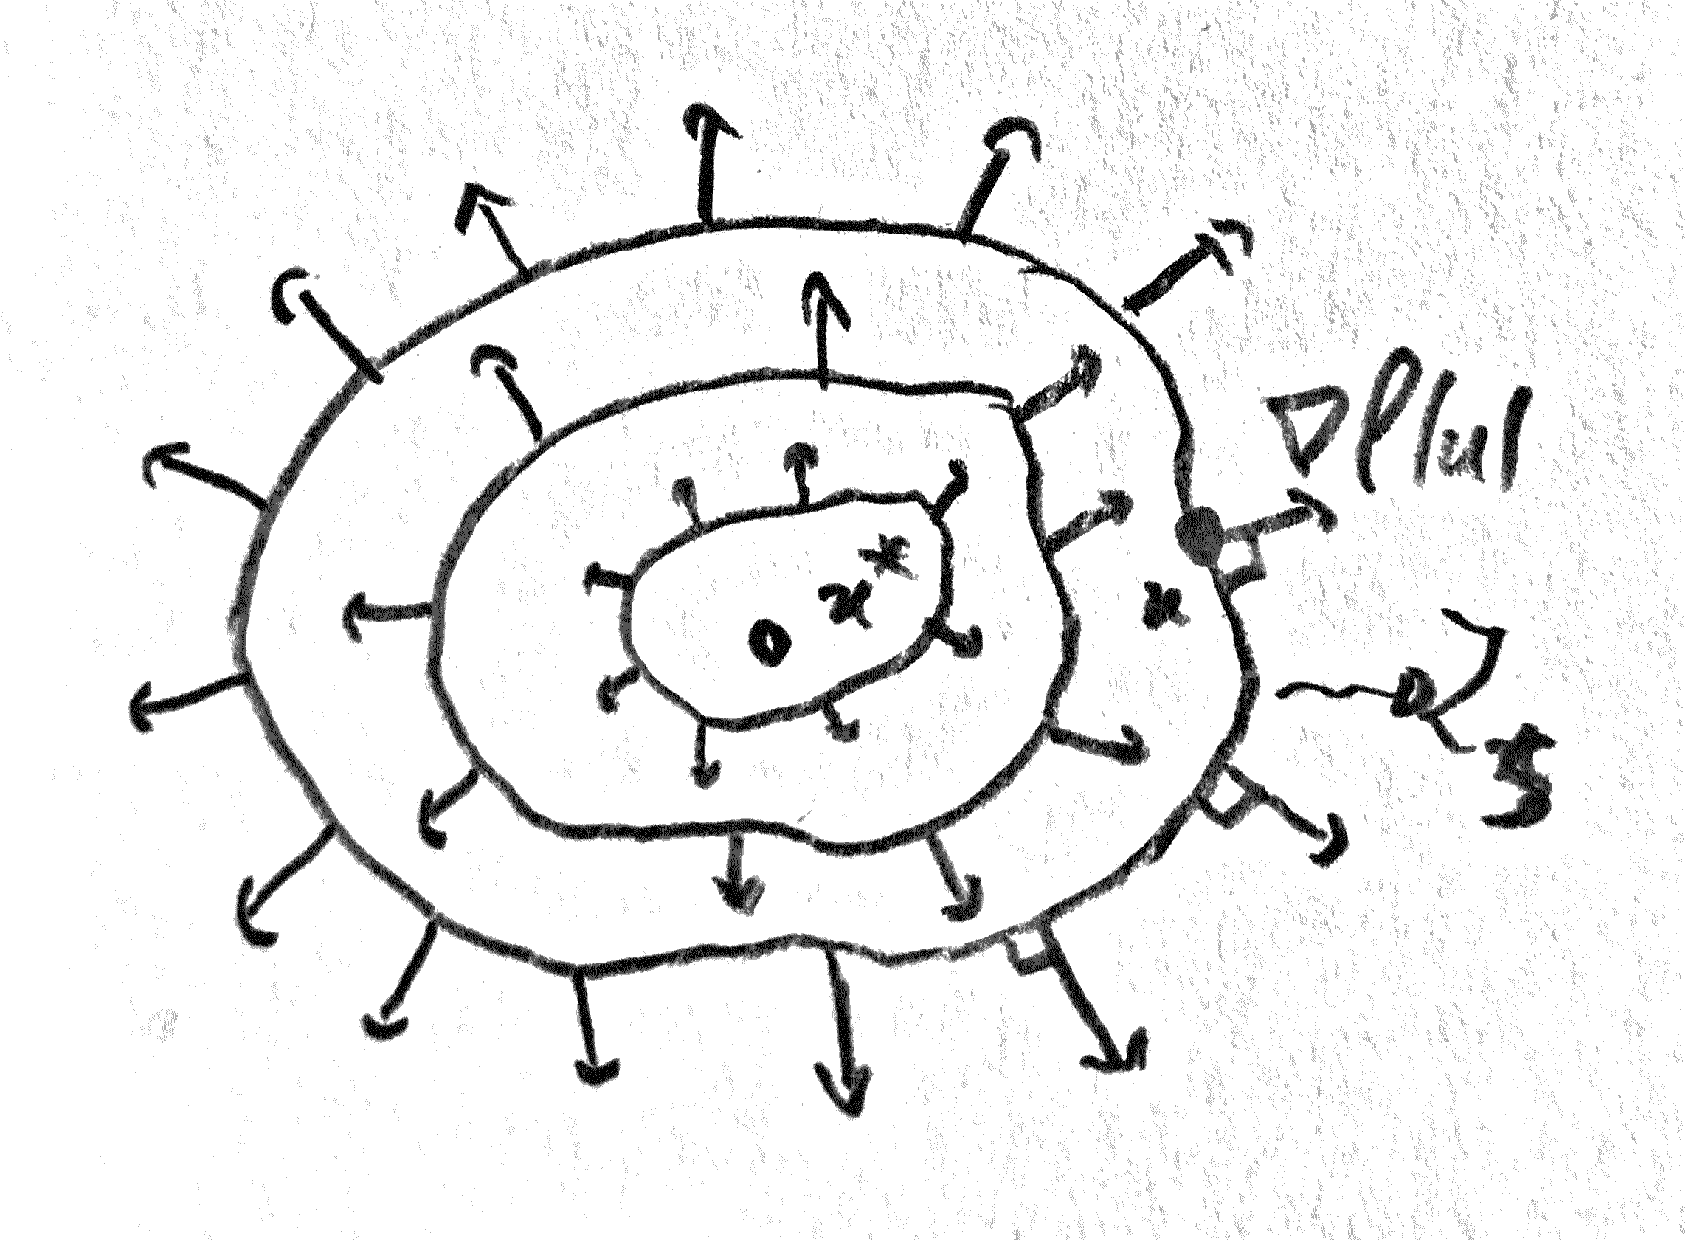
\includegraphics[width=.25\linewidth]{optim-smooth/level-sets-2} 
\caption{\label{fig-expansion-taylor}
	Left: First order Taylor expansion in 1-D and 2-D.
	Right: orthogonality of gradient and level sets and schematic of the proof.
}
\end{figure}

The gradient $\nabla f(x)$ should be understood as a direction along which the function increases. This means that to improve the value of the function, one should move in the direction $-\nabla f(x)$. Given some fixed $x$, let us look as the function $f$ along the 1-D half line 
\eq{ 
	\tau \in \RR^+ = [0,+\infty[ \longmapsto f(x-\tau \nabla f(x)) \in \RR.
}
If $f$ is differentiable at $x$, one has 
\eq{
	f(x-\tau \nabla f(x)) = f(x) - \tau \dotp{\nabla f(x)}{\nabla f(x)} + o(\tau)
		= f(x) - \tau \norm{\nabla f(x)}^2 + o(\tau).
}
So there are two possibility: either $\nabla f(x)=0$, in which case we are already at a minimum (possibly a local minimizer if the function is non-convex) or if $\tau$ is chosen small enough, 
\eq{
	f(x-\tau \nabla f(x)) < f(x)
} 
which means that moving from $x$ to $x-\tau \nabla f(x)$ has improved the objective function. 

\begin{rem}[Orthogonality to level sets]
	The level sets of $f$ are the sets of point sharing the same value of $f$, i.e. for any $s \in \RR$
	\eq{
		\Ll_s \eqdef \enscond{x}{f(x)=s}.		
	}
	At some $x \in \RR^p$, denoting $s=f(x)$, then $x \in \Ll_s$ ($x$ belong to its level set). The gradient vector $\nabla f(x)$ is orthogonal to the level set (as shown on Fig.~\ref{fig-expansion-taylor} right), and points toward level set of higher value (which is consistent with the previous computation showing that it is a valid ascent direction). 
	%
	Indeed, lets consider around $x$ inside $\Ll_s$ a smooth curve of the form $t \in \RR \mapsto c(t)$ where $c(0)=x$. 
	%	
	Then the function $h(t) \eqdef f(c(t))$ is constant $h(t)=s$  since $c(t)$ belong to the level set. So $h'(t)=0$. But at the same time, we can compute its derivate at $t=0$ as follow
	\eq{
		h(t) = f(c(0) + t c'(0) + o(t)) = h(0) + \de \dotp{c'(0)}{\nabla f(c(0))} + o(t)
	}	
	i.e. $h'(0) = \dotp{c'(0)}{\nabla f(x)}=0$, so that $\nabla f(x)$ is orthogonal to the tangent $c'(0)$ of the curve $c$, which lies in the tangent plane of $\Ll_s$  (as shown on Fig.~\ref{fig-expansion-taylor}, right).  Since the curve $c$ is arbitrary, the whole tangent plane is thus orthogonal to $\nabla f(x)$. 
\end{rem}

\begin{rem}[Local optimal descent direction]
	One can prove something even stronger, that among all possible direction $u$ with $\norm{u}=r$, $r \frac{\nabla f(x)}{\norm{\nabla f(x)}}$ becomes the optimal one as $r \rightarrow 0$ (so for very small step this is locally the best choice), more precisely, 
\eq{
	\frac{1}{r} \uargmin{\norm{u}=r} f(x + u) \overset{r \rightarrow 0}{\longrightarrow} -\frac{\nabla f(x)}{\norm{\nabla f(x)}}.
}
Indeed, introducing a Lagrange multiplier $\la \in \RR$ for this constraint optimization problem, one obtains that the optimal $u$ satisfies $\nabla f(x+u) = \la u$ and $\norm{u}=r$. Thus $\frac{u}{r} =\pm \frac{\nabla f(x+u)}{\norm{\nabla f(x+u)}}$, and assuming that $\nabla f$ is continuous, when $\norm{u}=r \rightarrow 0$, this converges to $\frac{u}{\norm{u}} = \pm\frac{\nabla f(x)}{\norm{\nabla f(x)}}$. The sign $\pm$ should be $+1$ to obtain a maximizer and $-1$ for the minimizer.
\end{rem}


%%%%%%%%%%%%%%%%%%%%%%%%%%%%%%%%%%%%%%%%%%%%%%%%%%%%%%%%%%%%%%%%%%%%%%%%%%%%%%%%%%
\subsection{Gradient Descent}

The gradient descent algorithm reads, starting with some $x_0 \in \RR^p$
\eql{\label{eq-grad-desc}
	x_{k+1} \eqdef x_k - \tau_k \nabla f(x_k)
}
where $\tau_k>0$ is the step size (also called learning rate). For a small enough $\tau_k$, the previous discussion shows that the function $f$ is decaying through the iteration. So intuitively, to ensure convergence, $\tau_k$ should be chosen small enough, but not too small so that the algorithm is as fast as possible.
%
In general, one use a fix step size $\tau_k=\tau$, or try to adapt $\tau_k$ at each iteration (see Fig.~\ref{fig-gradesc}). 


\begin{figure}
\centering
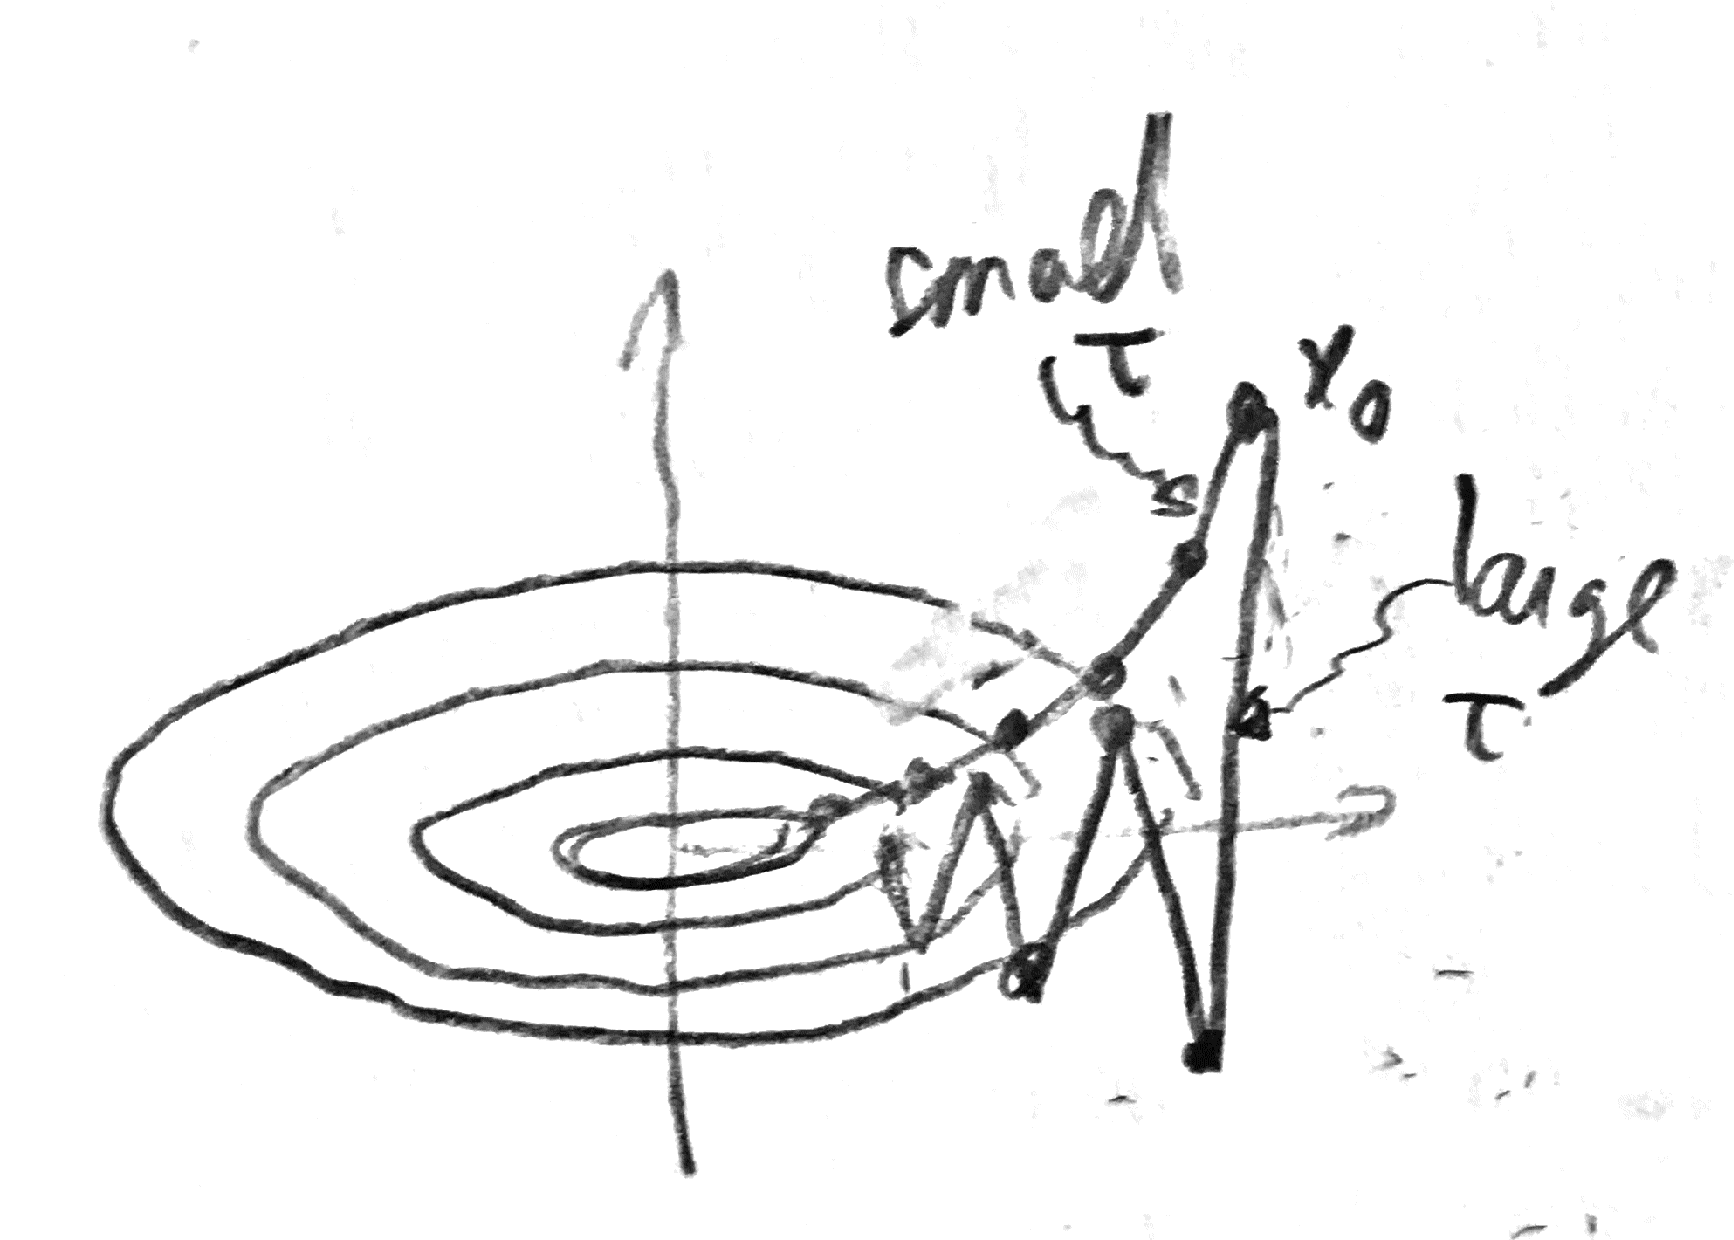
\includegraphics[width=.3\linewidth]{optim-smooth/grad-desc-1} \quad
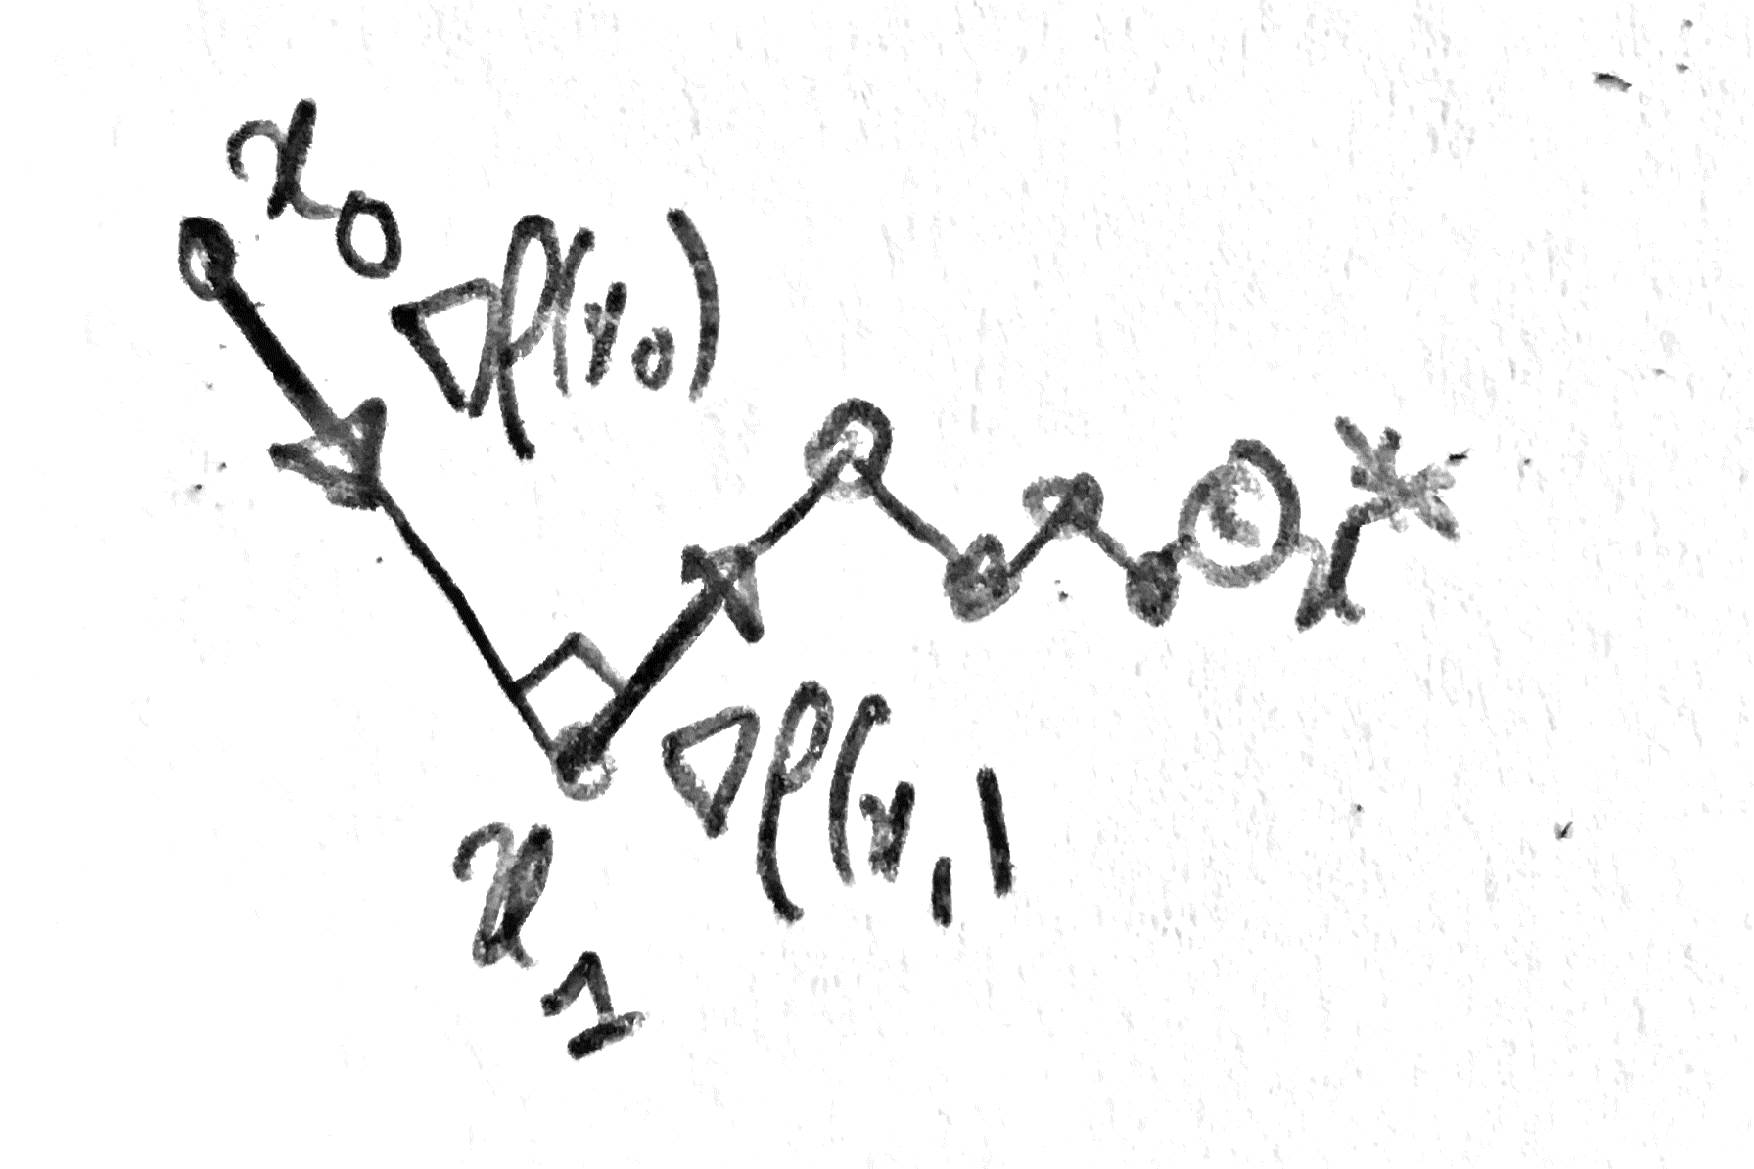
\includegraphics[width=.3\linewidth]{optim-smooth/grad-desc-2} 
\caption{\label{fig-gradesc}
Influence of $\tau$ on the gradient descent (left) and optimal step size choice (right).
}
\end{figure}


\begin{rem}[Greedy choice]
Although this is in general too costly to perform exactly, one can use a ``greedy'' choice, where the step size is optimal at each iteration, i.e. 
\eq{
	\tau_k \eqdef \uargmin{\tau} h(\tau) \eqdef f(x_k-\tau \nabla f(x_k)).
}
Here $h(\tau)$ is a function of a single variable. One can compute the derivative of $h$ as
\eq{
	h(\tau+\de) = f(x_k-\tau \nabla f(x_k) - \de \nabla f(x_k)) = f(x_k-\tau \nabla f(x_k))- \dotp{\nabla f(x_k-\tau \nabla f(x_k))}{ \nabla f(x_k)} + o(\de).
}
One note that at $\tau=\tau_k$, $\nabla f(x_k-\tau \nabla f(x_k))=\nabla f(x_{k+1})$ by definition of $x_{k+1}$ in~\eqref{eq-grad-desc}. 
%
Such an optimal $\tau=\tau_k$ is thus characterized by
\eq{
	h'(\tau_k) = - \dotp{\nabla f(x_k)}{\nabla f(x_{k+1})} = 0.
}
This means that for this greedy algorithm, two successive descent direction $\nabla f(x_k)$ and $\nabla f(x_{k+1})$ are orthogonal (see Fig.~\ref{fig-gradesc}).
\end{rem}




%%%%%%%%%%%%%%%%%%%%%%%%%%%%%%%%%%%%%%%%%%%%%%%%%%%%%%%%%%%%%%%%%%%%%%%%%%%%%%%%%%
%%%%%%%%%%%%%%%%%%%%%%%%%%%%%%%%%%%%%%%%%%%%%%%%%%%%%%%%%%%%%%%%%%%%%%%%%%%%%%%%%%
%%%%%%%%%%%%%%%%%%%%%%%%%%%%%%%%%%%%%%%%%%%%%%%%%%%%%%%%%%%%%%%%%%%%%%%%%%%%%%%%%%
\section{Convergence Analysis}


%%%%%%%%%%%%%%%%%%%%%%%%%%%%%%%%%%%%%%%%%%%%%%%%%%%%%%%%%%%%%%%%%%%%%%%%%%%%%%%%%%
\subsection{Quadratic Case}

%%%
\paragraph{Convergence analysis for the quadratic case.}

We first analyze this algorithm in the case of the quadratic loss, which can be written as
\eq{
	f(x) = \frac{1}{2}\norm{Ax-y}^2 = \frac{1}{2} \dotp{Cx}{x} - \dotp{x}{b} + \text{cst}
	\qwhereq
	\choice{
		C \eqdef A^\top A \in \RR^{p \times p}, \\
		b \eqdef A^\top y \in \RR^p. 
	}	
} 
We already saw that in~\eqref{eq-sol-leastsquare} if $\ker(A)=\{0\}$, which is equivalent to $C$ being invertible, then there exists a single global minimizer $x^\star = (A^\top A)^{-1} A^\top y = C^{-1} u$. 

Note that a function of the form $\frac{1}{2} \dotp{Cx}{x} - \dotp{x}{b}$ is convex if and only if the symmetric matrix $C$ is positive semi-definite, i.e. that all its eigenvalues are non-negative (as already seen in~\eqref{eq-pca-decomp}).

\begin{prop}\label{prop-graddesc-quad}
	For $f(x)=\dotp{Cx}{x}-\dotp{b}{x}$ ($C$ being symmetric semi-definite positive) with the eigen-values of $C$ upper-bounded by $L$ and lower-bounded by $\mu>0$, assuming there exists $(\tau_{\min},\tau_{\max})$ such that
	\eq{
		0 < \tau_{\min} \leq \tau_\ell \leq \tilde\tau_{\max} < \frac{2}{L}
	}
	then there exists $0 \leq \tilde\rho<1$ such that 
	\eql{\label{eq-global-linrate-grad}
		\norm{ x_k-x^\star } \leq \tilde\rho^\ell \norm{x_0-x^\star}.
	} 
	The best rate $\tilde\rho$ is obtained for 
	\eql{\label{eq-best-rate-local}
		\tau_\ell = \frac{2}{L+\mu}
		\qarrq
		\tilde\rho \eqdef \frac{L-\mu}{L+\mu} = 1 - \frac{2\epsilon}{1+\epsilon}
		\qwhereq
		\epsilon \eqdef \mu/L.
	} 
\end{prop}
\begin{proof}
	One iterate of gradient descent reads 
	\eq{
		x_{k+1}=x_k-\tau_\ell (C x_k-b).
	}	
	Since the solution $x^\star$ (which by the way is unique by strict convexity) satisfy the first order condition $C x^\star=b$, it gives
	\eq{
		x_{k+1}-x^\star =x_k-x^\star-\tau_\ell C(x_k-x^\star) = (\Id_p-\tau_\ell C)(x_k-x^\star).
	}	
	%	
	If $S \in \RR^{p \times p}$ is a symmetric matrix, one has 
	\eq{
		\norm{Sz} \leq \norm{S}_{\text{op}}  \norm{z}
		\qwhereq
		\norm{S}_{\text{op}} \eqdef \max_k |\la_k(S)|, 
	}
	where $\la_k(S)$ are the eigenvalues of $S$ and $\si_k(S) \eqdef |\la_k(S)|$ are its singular values.
	%
	Indeed, $S$ can be diagonalized in an orthogonal basis $U$, so that $S=U \diag(\la_k(S)) U^\top$,
	and $S^\top S = S^2 = U \diag(\la_k(S)^2) U^\top$ so that 
	\begin{align*}
		\norm{Sz}^2 &= \dotp{S^\top S z}{z} = \dotp{U \diag(\la_k) U^\top z}{z}		 
		=\dotp{\diag(\la_k^2) U^\top z}{U^\top z} \\
		&= \sum_i \la_k^2 (U^\top z)_k^2 \leq \max_k(\la_k^2) \norm{U^\top z}^2
		= \max_k(\la_k^2) \norm{z}^2.
	\end{align*}
	
	Applying this to $S = \Id_p-\tau_\ell C$, one has
	\eq{
		h(\tau) \eqdef \norm{\Id_p-\tau_\ell C}_{\text{op}} = \max_k |\la_k(\Id_p-\tau_\ell C)|
		= \max_k |1-\tau_\ell \la_k(C)|
		= \max( |1-\tau_\ell \si_{\max}(C)|,|1-\tau \si_{\min}(C)| )
	}
	For a quadratic function, one has $\si_{\min}(C) = \mu, \si_{\max}(C)=L$. Figure~\ref{fig-grad-desc-contract}, right, shows a display of $h(\tau)$. One has that for $0<\tau<2/L$, $h(\tau)<1$.
	%
	The optimal value is reached at $\tau^\star = \frac{2}{L+\mu}$ and then 
	\eq{
		h(\tau^\star) = \left|.1 - \frac{2L}{L+\mu} \right| = \frac{L-\mu}{L+\mu}.
	}
\end{proof}



\begin{figure}
\centering
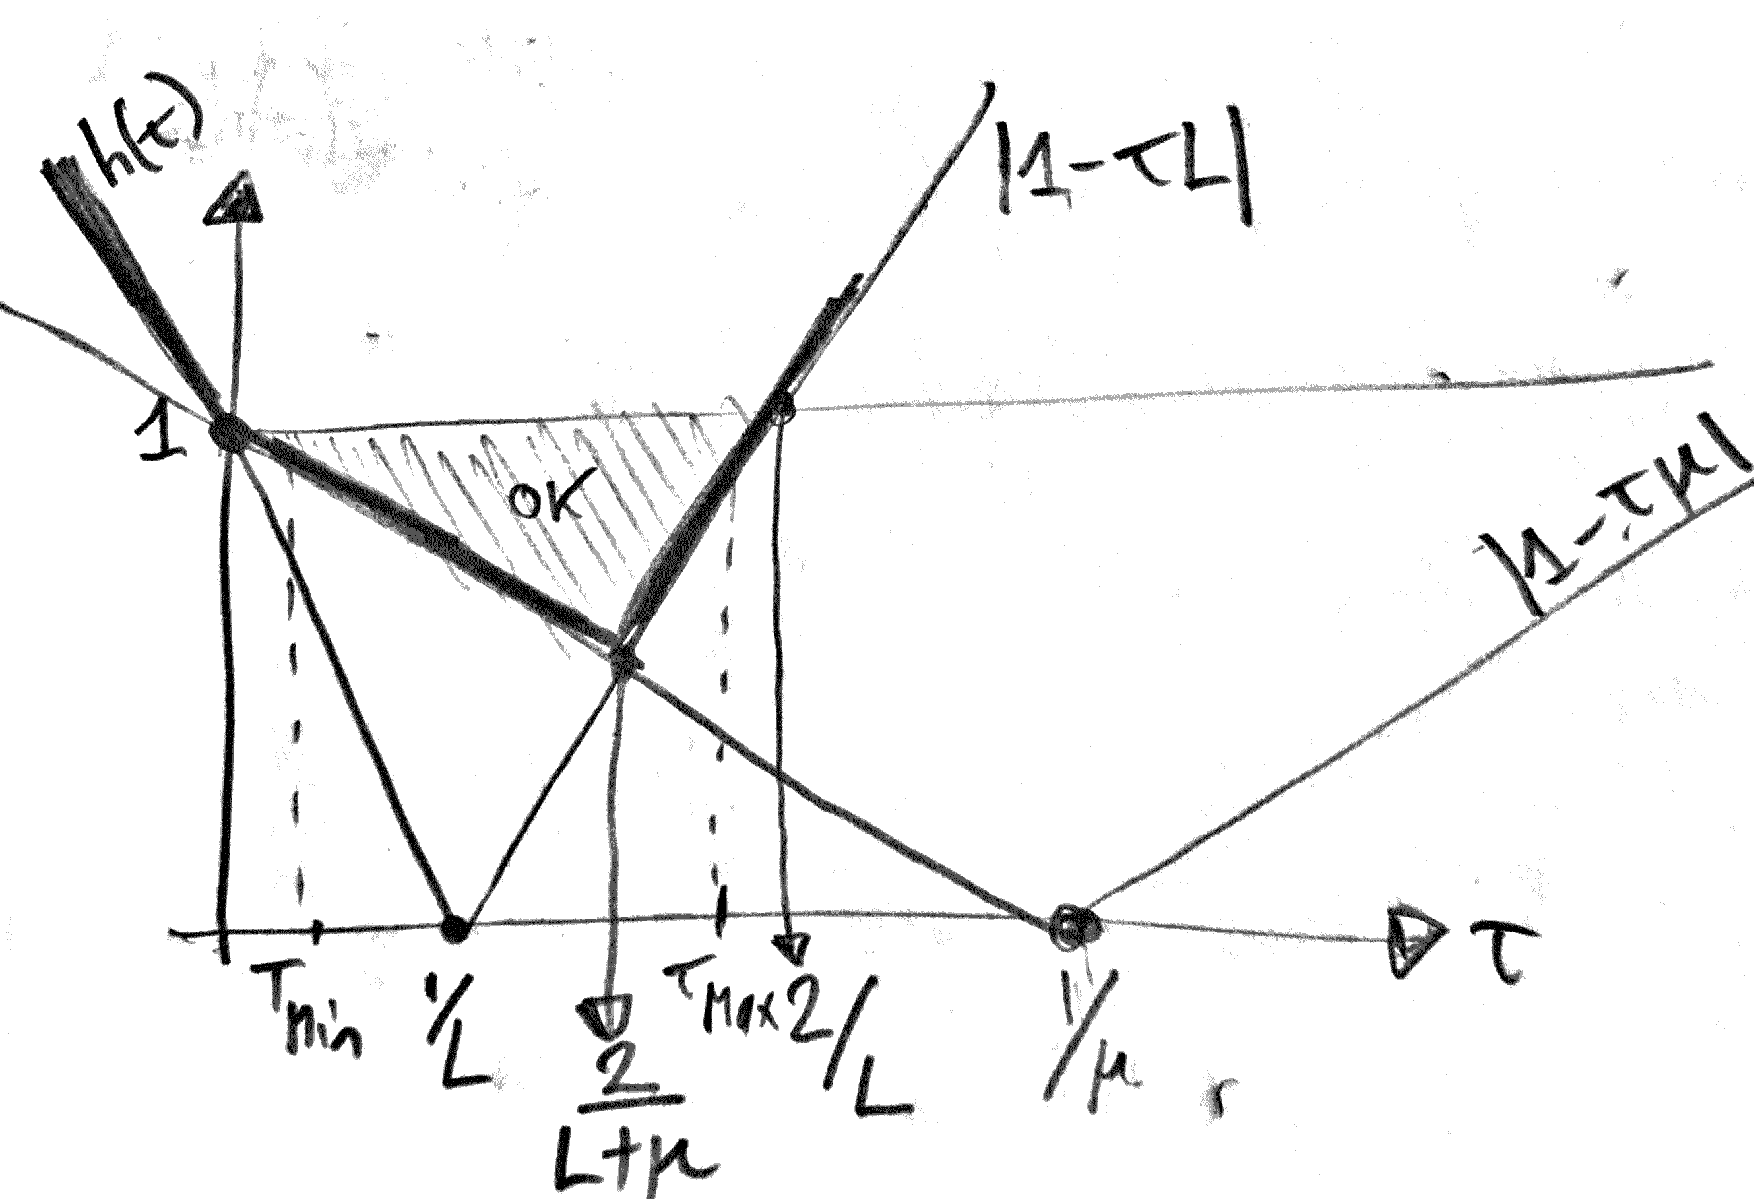
\includegraphics[width=.35\linewidth]{optim-smooth/proof-quadr}
\caption{\label{fig-grad-desc-contract}
Contraction constant $h(\tau)$ for a quadratic function (right). 
}
\end{figure}

Note that when the condition number $\xi \eqdef \mu/L \ll 1$
is small (which is the typical setup for ill-posed problems), then the contraction constant appearing in~\eqref{eq-best-rate-local} scales like 
\eql{\label{eq-rate-strong-quad}
	\tilde\rho \sim 1-2\xi.
}
%
The quantity $\epsilon$ in some sense reflects the inverse-conditioning of the problem. For quadratic function, it indeed corresponds exactly to the inverse of the condition number (which is the ratio of the largest to smallest singular value). The condition number is minimum and equal to $1$ for orthogonal matrices.

The error decay rate~\eqref{eq-global-linrate-grad}, although it is geometrical $O(\rho^k)$ is called a ``linear rate'' in the optimization literature. It is a ``global'' rate because it hold for all $k$ (and not only for large enough $k$).

If $\ker(A) \neq \{0\}$, then $C$ is not definite positive (some of its eigenvalues vanish), and the set of solution is infinite. 
%
One can however still show a linear rate, by showing that actually the iterations $x_k$ are orthogonal to $\ker(A)$ and redo the above proof replacing $\mu$ by the smaller non-zero eigenvalue of $C$. This analysis however leads to a very poor rate $\rho$ (very close to 1) because $\mu$ can be arbitrary close to 0. Furthermore, such a proof does not extends to non-quadratic functions. It is thus necessary to do a different theoretical analysis, which only shows a sublinear rate on the objective function $f$ itself rather than on the iterates $x_k$.  

\begin{prop}\label{prop-graddesc-quad-sublin}
	For $f(x)=\dotp{Cx}{x}-\dotp{b}{x}$, assuming the eigenvalue of $C$ are bounded by $L$, then if $0<\tau_k=\tau < 2/L$ is constant, then
	\eq{
		f(x_k)-f(x^\star) \leq \frac{\text{\upshape dist}(x_0,\argmin f)^2}{\tau 8 k}.
	}
	where 
	\eq{
		\text{\upshape dist}(x_0,\argmin f) \eqdef \umin{x^\star \in \argmin f} \norm{x_0-x^\star}.
	}
\end{prop}
\begin{proof}	
	We have $C x^\star=b$ for any minimizer $x^\star$
	and $x_{k+1}=x_k-\tau (C x_k-b)$ so that as before
	\eq{
		x_k-x^\star = (\Id_p-\tau C)^k(x_0-x^\star).
	}
	Now one has
	\eq{
		\frac{1}{2}\dotp{C(x_k-x^\star}{x_k-x^\star} = 
		\frac{1}{2}\dotp{Cx_k}{x_k} 
		- \dotp{Cx_k}{x^\star}
		+ \frac{1}{2} \dotp{Cx^\star}{x^\star}
	}
	and we have $\dotp{Cx_k}{x^\star} = \dotp{x_k}{Cx^\star} = \dotp{x_k}{b}$
	and also $\dotp{Cx^\star}{x^\star} = \dotp{x^\star}{x}$ so that
	\eq{
		\frac{1}{2}\dotp{C(x_k-x^\star}{x_k-x^\star} = 
		\frac{1}{2}\dotp{Cx_k}{x_k} - \dotp{x_k}{b}
		+ \frac{1}{2} \dotp{x^\star}{b}
		= f(x_k)-f(x^\star)
	}
	where we have used the fact that
	\eq{
		f(x^\star) = \frac{1}{2}\dotp{(A^\top A) (A^\top A)^{-1} b}{(A^\top A)^{-1} b} - \dotp{(A^\top A)^{-1} b}{b}
		\qarrq
		\frac{1}{2} \dotp{x^\star}{b} = -f(x^\star).	
	}
	This thus implies 
	\eq{
		f(x_k)-f(x^\star) = 
		\frac{1}{2}\dotp{(\Id_p-\tau C)^k C (\Id_p-\tau C)^k (x_0-x^\star)}{x_0-x^\star}
		\leq \frac{\si_{\max}(M_k)}{2} \umin{x^\star} \norm{x_0-x^\star}^2
	}
	where we have denoted
	\eq{
		M_k \eqdef (\Id_p-\tau C)^k C (\Id_p-\tau C)^k.
	}
	One has 
	\eq{
		\si_\ell(M_k) = \si_\ell(C) (1-\tau \si_\ell(C))^{2k}
			\leq \frac{1}{\tau 4 k}
	}
	since one can show that (setting $t = \tau \si_\ell(C) \leq 1$ because of the hypotheses)
	\eq{
		\foralls t \in [0,1], \quad
			(1-t)^{2k} t \leq \frac{1}{4k}.
	}
	Indeed, one has
	\begin{align*}
		(1-t)^{2k} t \leq (e^{-t})^{2k}t
		= \frac{1}{2k} (2kt) e^{-2k t}
		\leq \frac{1}{2k} \usup{u \geq 0} u e^{-u}
		= \frac{1}{2e k} \leq \frac{1}{4k}.
	\end{align*}
\end{proof}	
	



%%%%%%%%%%%%%%%%%%%%%%%%%%%%%%%%%%%%%%%%%%%%%%%%%%%%%%%%%%%%%%%%%%%%%%%%%%%%%%%%%%
\subsection{General Case}

We detail the theoretical analysis of convergence for general smooth convex functions. 
%
The general idea is to replace the linear operator $C$ involved in the quadratic case by the second order derivative (the hessian matrix).  

%%%
\paragraph{Hessian.}

If the function is twice differentiable along the axes, the hessian matrix is 
\eq{
	(\partial^2 f)(x) = \pa{ \frac{\partial^2 f(x)}{\partial x_i \partial x_j} }_{1 \leq i,j \leq p} \in \RR^{p \times p}.
}	
Where recall that $\frac{\partial^2 f(x)}{\partial x_i \partial x_j}$ is the differential along direction $x_j$ of the function $x \mapsto \pd{f(x)}{x_i}$. We also recall that $\frac{\partial^2 f(x)}{\partial x_i \partial x_j} = \frac{\partial^2 f(x)}{\partial x_j \partial x_i}$ so that $\partial^2 f(x)$ is a symmetric matrix.

A differentiable function $f$ is said to be twice differentiable at $x$ if
\eql{\label{eq-taylor-hess}
	f(x+\epsilon) = f(x) + \dotp{\nabla f(x)}{\epsilon} + \frac{1}{2} \dotp{\partial^2 f(x) \epsilon}{\epsilon}
	+ o(\norm{\epsilon}^2).
}
This means that one can approximate $f$ near $x$ by a quadratic function. 
%
The hessian matrix is uniquely determined by this relation, so that if one is able to write down an expansion with some matrix $H$
\eq{
	f(x+\epsilon) = f(x) + \dotp{\nabla f(x)}{\epsilon} + \frac{1}{2} \dotp{H \epsilon}{\epsilon}
	+ o(\norm{\epsilon}^2).
}
then equating this with the expansion~\eqref{eq-taylor-hess} ensure that $\partial^2 f(x)=H$. This is thus a way to actually determine the hessian without computing all the $p^2$ partial derivative.
%
This Hessian can equivalently be obtained by performing an expansion (i.e. computing the differential) of the gradient since
\eq{
	\nabla f(x+\epsilon) = \nabla f(x) + [\partial^2 f(x)](\epsilon) + o(\norm{\epsilon})
}
where $[\partial^2 f(x)](\epsilon) \in \RR^p$ denotes the multiplication of the matrix $\partial^2 f(x)$ with the vector $\epsilon$. 

One can show that a twice differentiable function $f$ on $\RR^p$ is convex if and only if for all $x$ the symmetric matrix $\partial^2 f(x)$ is positive semi-definite, i.e. all its eigenvalues are non-negative. 
% 
Furthermore, if these eigenvalues are strictly positive then $f$ is strictly convex (but the converse is not true, for instance $x^4$ is strictly convex on $\RR$ but its second derivative vanishes at $x=0$). 

For instance, for a quadratic function $f(x)=\dotp{C x}{x} - \dotp{x}{u}$, one has $\nabla f(x) = Cx-u$ and thus $\partial^2 f(x) = C$ (which is thus constant).
%
For the classification function, one has 
\eq{
	\nabla f(x) = -A^\top \diag(y) \nabla L( -\diag(y) Ax). 
}
and thus
\begin{align*}
	\nabla f(x+\epsilon) &= -A^\top \diag(y) \nabla L( -\diag(y) Ax - -\diag(y) A\epsilon)  \\
		&= \nabla f(x)  -A^\top \diag(y) [\partial^2 L( -\diag(y) Ax)]( -\diag(y) A\epsilon) 
\end{align*}
Since $\nabla L(u) = (\ell'(u_i))$ one has $\partial^2 L(u)=\diag(\ell''(u_i))$. This means that 
\eq{
	\partial^2 f(x) = A^\top \diag(y) \times \diag( \ell''(-\diag(y) Ax) ) \times \diag(y) A.
}
One verifies that this matrix is symmetric and positive if $\ell$ is convex and thus $\ell''$ is positive. 

\begin{rem}[Second order optimality condition]
The first use of Hessian is to decide wether a point $x^\star$ with $\nabla f(x^\star)$ is a local minimum or not. Indeed, if $\partial^2 f(x^\star)$ is a positive matrix (i.e. its eigenvalues are strictly positive), then $x^\star$ is a strict local minimum. 
%
Note that if $\partial^2 f(x^\star)$ is only non-negative (i.e. some its eigenvalues might vanish) then one cannot deduce anything (such as for instance $x^3$ on $\RR$). 
%
Conversely, if $x^\star$ is a local minimum then $\partial^2 f(x)$
\end{rem}

\begin{rem}[Second order algorithms]
A second use, is to be used in practice to define second order method (such as Newton's algorithm), which converge faster than gradient descent, but are more costly. The generalized gradient descent reads
\eq{
	x_{k+1} = x_k - H_k \nabla f(x_k)
}
where $H_k \in \RR^{p \times p}$ is a positive symmetric matrix. One recovers the gradient descent when using $H_k=\tau_k \Id_p$, and Newton's algorithm corresponds to using the inverse of the Hessian $H_k=[\partial^2 f(x_k)]^{-1}$.
%
Note that
\eq{
	f(x_k) = f(x_k) - \dotp{H_k \nabla f(x_k)}{\nabla f(x_k)} + o(\norm{H_k \nabla f(x_k)}).
}
Since $H_k$ is positive, if $x_k$ is not a minimizer, i.e. $\nabla f(x_k) \neq 0$, then $\dotp{H_k \nabla f(x_k)}{\nabla f(x_k)}>0$.
%
So if $H_k$ is small enough one has a valid descent method in the sense that $f(x_{k+1}) < f(x_k)$.
%
It is not the purpose of this chapter to explain in more detail these type of algorithm.
\end{rem}

The last use of Hessian, that we explore next, is to study theoretically the convergence of the gradient descent. One simply needs to replace the boundedness of the eigenvalue of $C$ of a quadratic function by a boundedness of the eigenvalues of $\partial^2 f(x)$ for all $x$.
%
Roughly speaking, the theoretical analysis of the gradient descent for a generic function is obtained by applying this approximation and using the proofs of the previous section.


%%%
\paragraph{Smoothness and strong convexity.}

\wrapfSimple{optim-smooth/up-low-bounds}
One also needs to quantify the smoothness of $f$. This is enforced by requiring that the gradient is $L$-Lipschitz, i.e.
\eql{\label{eq-lipsch-grad}\tag{$\Rr_L$}
	\foralls (x,x') \in (\RR^p)^2, \quad
	\norm{ \nabla f(x)-\nabla f(x') } \leq L \norm{x-x'}. 
}
In order to obtain fast convergence of the iterates themselve, it is needed that the function has enough ``curvature'' (i.e. is not too flat), which corresponds to imposing that $f$ is $\mu$-strongly convex
\eql{\label{eq-strong-conv}\tag{$\Ss_\mu$}
	\foralls (x,x'), \in (\RR^p)^2, \quad
	\dotp{\nabla f(x)-\nabla f(x')}{ x-x' } \geq \mu \norm{x-x'}^2. 
}
The following proposition express these conditions as constraints on the hessian for $\Cc^2$ functions.

\begin{prop}\label{prop-smooth-strong}
Conditions~\eqref{eq-lipsch-grad} and~\eqref{eq-strong-conv} imply
\eql{\label{eq-above-below-quad}
	\foralls (x,x'), \quad
	f(x') + \dotp{\nabla f(x)}{x'-x} + \frac{\mu}{2}\norm{x-x'}^2
	\leq
	f(x) 
	\leq 
	f(x') + \dotp{\nabla f(x')}{x'-x} + \frac{L}{2}\norm{x-x'}^2.
}
If $f$ is of class $\Cc^2$, conditions~\eqref{eq-lipsch-grad} and~\eqref{eq-strong-conv} are equivalent to
\eql{\label{eq-upper-lower-bound-hess}
	\foralls x, \quad \mu \Id_{p}  \preceq \partial^2 f(x) \preceq L \Id_{p}
}
where $\partial^2 f(x) \in \RR^{p \times p}$ is the Hessian of $f$, and 
where $\preceq$ is the natural order on symmetric matrices, i.e.
\eq{
	A \preceq B \quad\Longleftrightarrow\quad
	\foralls x \in \RR^p, \quad \dotp{A u}{u} \leq \dotp{B u}{u}.
}
\end{prop}

\begin{proof}
	We prove~\eqref{eq-above-below-quad}, using Taylor expansion with integral remain
	\eq{
		f(x') - f(x) = \int_0^1 \dotp{\nabla f(x_t)}{x'-x} \d t
		= \dotp{\nabla f(x)}{x'-x} + \int_0^1 \dotp{\nabla f(x_t)-\nabla f(x)}{x'-x} \d t		
	}
	where $x_t \eqdef x+t(x'-x)$.
	%
	Using Cauchy-Schwartz, and then the smoothness hypothesis~\eqref{eq-lipsch-grad}
	\eq{
		f(x') - f(x) \leq \dotp{\nabla f(x)}{x'-x} +  \int_0^1 L \norm{x_t-x} \norm{x'-x} \d t
		\leq \dotp{\nabla f(x)}{x'-x} +  L \norm{x'-x}^2 \int_0^1  t  \d t
	} 
	which is the desired upper-bound. Using directly~\eqref{eq-strong-conv} gives 
	\eq{
		f(x') - f(x) 
		= \dotp{\nabla f(x)}{x'-x} + \int_0^1 \dotp{\nabla f(x_t)-\nabla f(x)}{\frac{x_t-x}{t}} \d t	
		\geq \dotp{\nabla f(x)}{x'-x} + \mu \int_0^1 \frac{1}{t}\norm{x_t-x}^2  \d t
	}
	which gives the desired result since $\norm{x_t-x}^2 / t = t \norm{x'-x}^2$.
\end{proof}

The relation~\eqref{eq-above-below-quad} shows that a smooth (resp. strongly convex) functional is bounded by bellow (resp. above) by a quadratic tangential majorant (resp. minorant). 

Condition~\eqref{eq-upper-lower-bound-hess} thus reads that the singular values of $\partial^2 f(x)$ should be contained in the interval $[\mu,L]$. The upper bound is also equivalent to $\norm{\partial^2 f(x)}_{\text{op}} \leq L$ where $\norm{\cdot}_{\text{op}}$ is the operator norm, i.e. the largest singular value. 
%
In the special case of a quadratic function of the form $\dotp{Cx}{x}-\dotp{b}{x}$ (recall that necessarily $C$ is semi-definite symmetric positive for this function to be convex), $\partial^2 f(x)=C$ is constant, so that $[\mu,L]$ can be chosen to be the range of the eigenvalues of $C$.

%%%
\paragraph{Convergence analysis.}

We now give convergence theorem for a general convex function. On contrast to quadratic function, if one does not assumes strong convexity, one can only show a sub-linear rate on the function values (and no rate at all on the iterates themselves). It is only when one assume strong convexity that linear rate is obtained. 
%
Note that in this case, the solution of the minimization problem is not necessarily unique.

\begin{thm}\label{thm-gradsec-non-strong-conv}
	If $f$ satisfy conditions~\eqref{eq-lipsch-grad}, assuming there exists $(\tau_{\min},\tau_{\max})$ such that
	\eq{
		0 < \tau_{\min} \leq \tau_\ell \leq \tau_{\max} < \frac{2}{L}, 
	}
	then $x_k$ converges to a solution $x^\star$ of~\eqref{eq-general-pbm} and
	there exists $C>0$ such that 
	\eql{\label{eq-sublin-rate-gd}
		f(x_k)-f(x^\star) \leq \frac{C}{\ell+1}.
	} 
	If furthermore $f$ is $\mu$-strongly convex, then there exists $0 \leq \rho < 1$ such that $\norm{x_k-x^\star} \leq \rho^\ell \norm{x_0-x^\star}$.
\end{thm}

\begin{proof}
	In the case where $f$ is not strongly convex, we only prove~\eqref{eq-sublin-rate-gd} since the proof that $x_k$ converges is more technical. Note indeed that if the minimizer $x^\star$ is non-unique, then it might be the case that the iterate $x_k$ ``cycle'' while approaching the set of minimizer, but actually convexity of $f$ prevents this kind of pathological behavior. 
	%
	For simplicity, we do the proof in the case $\tau_\ell = 1/L$, but it extends to the general case. 
	%
	The $L$-smoothness property imply~\eqref{eq-above-below-quad}, which reads
	\eq{
	f(x_{k+1}) 
		\leq 
		f(x_k) + \dotp{\nabla f(x_k)}{x_{k+1}-x_k} + \frac{L}{2}\norm{x_{k+1}-x_k}^2.
	}
	Using the fact that $x_{k+1}-x_k = -\frac{1}{L} \nabla f(x_k)$, one obtains
	\eql{\label{eq-proox-x'rad-nonstrong-1}
		f(x_{k+1}) 
		\leq 
		f(x_k) -  \frac{1}{L} \norm{\nabla f(x_k)}^2 + \frac{1}{2L} \norm{\nabla f(x_k)}^2
		\leq  f(x_k) -  \frac{1}{2L} \norm{\nabla f(x_k)}^2 
	}
	This shows that $(f(x_k))_\ell$ is a decaying sequence.
	%
	By convexity
	\eq{
		f(x_k) + \dotp{\nabla f(x_k)}{x^\star-x_k} \leq f(x^\star)
	}
	and plugging this in~\eqref{eq-proox-x'rad-nonstrong-1} shows
	\begin{align}
		f(x_{k+1})  &\leq   
		f(x^\star) - \dotp{\nabla f(x_k)}{x^\star-x_k} - \frac{1}{2L} \norm{\nabla f(x_k)}^2 \\
		&= f(x^\star) + \frac{L}{2}\pa{
			\norm{x_k-x^\star}^2 - \norm{x_k-x^\star-\frac{1}{L}\nabla f(x_k)}^2
		}\\
		&= f(x^\star) + \frac{L}{2}\pa{
			\norm{x_k-x^\star}^2 - \norm{x^\star-x_{k+1}}^2 }. \label{eq-conv-rate-proof-1}
	\end{align}
	Summing these inequalities for $\ell=0,\ldots,k$, one obtains
	\eq{
		\sum_{\ell=0}^k f(x_{k+1}) - (k+1) f(x^\star) \leq  \frac{L}{2}\pa{
			\norm{x_0-x^\star}^2 - \norm{x^{(k+1)}-x^\star}^2 }
	}
	and since $f(x_{k+1})$ is decaying $\sum_{\ell=0}^k f(x_{k+1}) \geq (k+1) f(x^{(k+1)})$, thus 
	\eq{
		f(x^{(k+1)}) - f(x^\star) \leq \frac{L \norm{x_0-x^\star}^2}{2(k+1)}
	}
	which gives~\eqref{eq-sublin-rate-gd} for $C \eqdef L \norm{x_0-x^\star}^2/2$.
	
	If we now assume $f$ is $\mu$-strongly convex, then, using $\nabla f(x^\star)=0$, one has $\frac{\mu}{2}\norm{x^\star-x}^2 \leq f(x)-f(x^\star)$ for all $x$. 
	%
	Re-manipulating~\eqref{eq-conv-rate-proof-1} gives
	\eq{
		\frac{\mu}{2}\norm{ x_{k+1} - x^\star}^2 \leq f(x_{k+1})-f(x^\star) \leq \frac{L}{2}\pa{
			\norm{x_k-x^\star}^2 - \norm{x^\star-x_{k+1}}^2 }, 
	}
	and hence
	\eql{\label{eq-rate-strong}
		\norm{ x_{k+1} - x^\star} \leq \sqrt{ \frac{L}{L+\mu} } \norm{ x_{k+1} - x^\star}, 
	}
	which is the desired result. 
\end{proof}

Note that in the low conditioning setting $\epsilon \ll 1$, one retrieve a dependency of the rate~\eqref{eq-rate-strong} similar to the one of quadratic functions~\eqref{eq-rate-strong-quad}, indeed 
\eq{
	\sqrt{ \frac{L}{L+\mu} } = (1+\epsilon)^{-\frac{1}{2}} \sim 1 - \frac{1}{2}\epsilon. 
}